% !TEX root = ../main.tex

\chapter{Implementation}
\label{ch:implementation}

\scaffold{
  \textbf{Overview paragraph} (writing guide, section 3.5). The reader knows the measurement principle from \cref{ch:measurement-principle}. Introduce the blocks of \cref{fig:block-diagram} with one sentence each, in signal-flow order: four jacks with four switched contacts each (tip, ring, sleeve, tip switch); per jack a shift register driving two analog switches that connect each contact to a shared pull-up or pull-down resistor; an RC filter per contact; two 24-bit ADCs, each reading two jacks; the Raspberry Pi Pico~2~W running the firmware; and the three outputs, USB MIDI to the host, an LED per jack and a WiFi access point serving the web interface. Then one sentence on the development method: the solver and the per-jack state machine live in a library without hardware dependencies that is tested on the host; the hardware drivers and the scheduling live in the firmware crate.
}

\begin{figure}[htbp]
  \centering
  \placeholderfigure{
    \textbf{Content.} Block diagram of the system, left to right: 4 jacks (J2--J5, contacts T, R, S, TS) $\rightarrow$ per jack: 74HC595 + 2$\times$TMUX1511 + shared \qty{1}{\kilo\ohm} pull-up to \qty{2.5}{\volt} and pull-down to GND $\rightarrow$ 16$\times$ RC filter (\qty{10}{\kilo\ohm}, \qty{10}{\nano\farad}) $\rightarrow$ 2$\times$ AD7718 (jacks 1--2 / 3--4, SPI0) $\rightarrow$ Raspberry Pi Pico~2~W (shift registers on SPI1) $\rightarrow$ USB MIDI, 4$\times$ WS2812B LED (GPIO6, level shifter), WiFi access point with web interface. Power block below: barrel jack $\rightarrow$ protection $\rightarrow$ LDOs \qty{5}{\volt}, \qty{3.3}{\volt}, \qty{2.5}{\volt} (from \qty{3.3}{\volt}); mark the \qty{2.5}{\volt} rail as both pull-up rail and ADC reference.

    \textbf{Focus.} Highlight (color) the analog measurement path of one jack; draw the other three jacks collapsed. Use the counts from \code{src/board.rs}.

    \textbf{How to obtain.} Draw in TikZ or a vector tool; style consistent with \code{docs/diagrams/}.
  }
  \titledcaption{System Block Diagram}{\scaffoldinline{One sentence per block group and the meaning of the highlighted path.}}
  \label{fig:block-diagram}
\end{figure}

% !TEX root = ../main.tex

\section{Design History and Decisions}
\label{sec:design-history}

\scaffold{
  \textbf{Paragraph 1, purpose of the section.} The hardware went through four stages: the project proposal (April 2026) \cite{benson2026proposal}, the circuit of milestone~1, a breadboard prototype (August 2026) and the final PCB (designed late August to early September 2026, assembled end of September). \Cref{tab:design-history} compares them; the following paragraphs give the reason for every change. The reader should finish the section knowing why the final board looks as it does, so that \crefrange{sec:analog-front-end}{sec:pcb} can describe it without justifying it again. Write in the past tense (events of the project), as the writing guide prescribes for findings.
}

\begin{table}[htbp]
  \centering
  \small
  \titledcaption{Design Stages}{\scaffoldinline{Explain the four columns (proposal \cite{benson2026proposal}, milestone~1 circuit, breadboard prototype, final PCB) and that the text gives the reason for each change. Cells marked [?] are unconfirmed.}}
  \label{tab:design-history}
  \begin{tabularx}{\linewidth}{@{}>{\raggedright\arraybackslash}p{0.15\linewidth}*{4}{>{\raggedright\arraybackslash}X}@{}}
    \toprule
    & \textbf{Proposal} & \textbf{Milestone 1} & \textbf{Breadboard} & \textbf{Final PCB} \\
    \midrule
    Microcontroller & STM32G4 or RP2040 & Pico~2 module & Pico~2~W & Pico~2~W \\
    ADC & ADS8688, 16-bit SAR & AD7124-8, 24-bit $\Sigma\Delta$ & AD7718 [?] & 2$\times$ AD7718, 24-bit $\Sigma\Delta$ \\
    Pull switching & TS5A23157 SPDT switches & SN74LVC126A tristate buffers & tristate buffers [?] & TMUX1511 SPST switches \\
    Pull resistance & series resistor per contact & \qty{1}{\kilo\ohm} per contact & \qty{1}{\kilo\ohm} per contact & \qty{1}{\kilo\ohm} \qty{0.1}{\percent}, shared per rail and jack \\
    Input filter & RC & \qty{1}{\kilo\ohm}, \qty{100}{\nano\farad} & \qtyrange{68}{100}{\nano\farad} [?] & \qty{10}{\kilo\ohm}, \qty{10}{\nano\farad} \\
    Contacts per jack & 3 & 4 (one unused) & 3 & 4 (tip switch used) \\
    Analog rail, reference & separate analog rail & \qty{3.3}{\volt} analog rail & \qty{3.3}{\volt} & \qty{2.5}{\volt} LDO, pull-up rail and reference \\
    Ground & star point & star point & -- & one ground net \\
    Outputs & USB MIDI, optional DIN MIDI & USB MIDI & USB MIDI, WiFi & USB MIDI, WiFi, 4 LEDs \\
    \bottomrule
  \end{tabularx}
\end{table}

\begin{figure}[htbp]
  \centering
  \begin{subfigure}[t]{\linewidth}
    \centering
    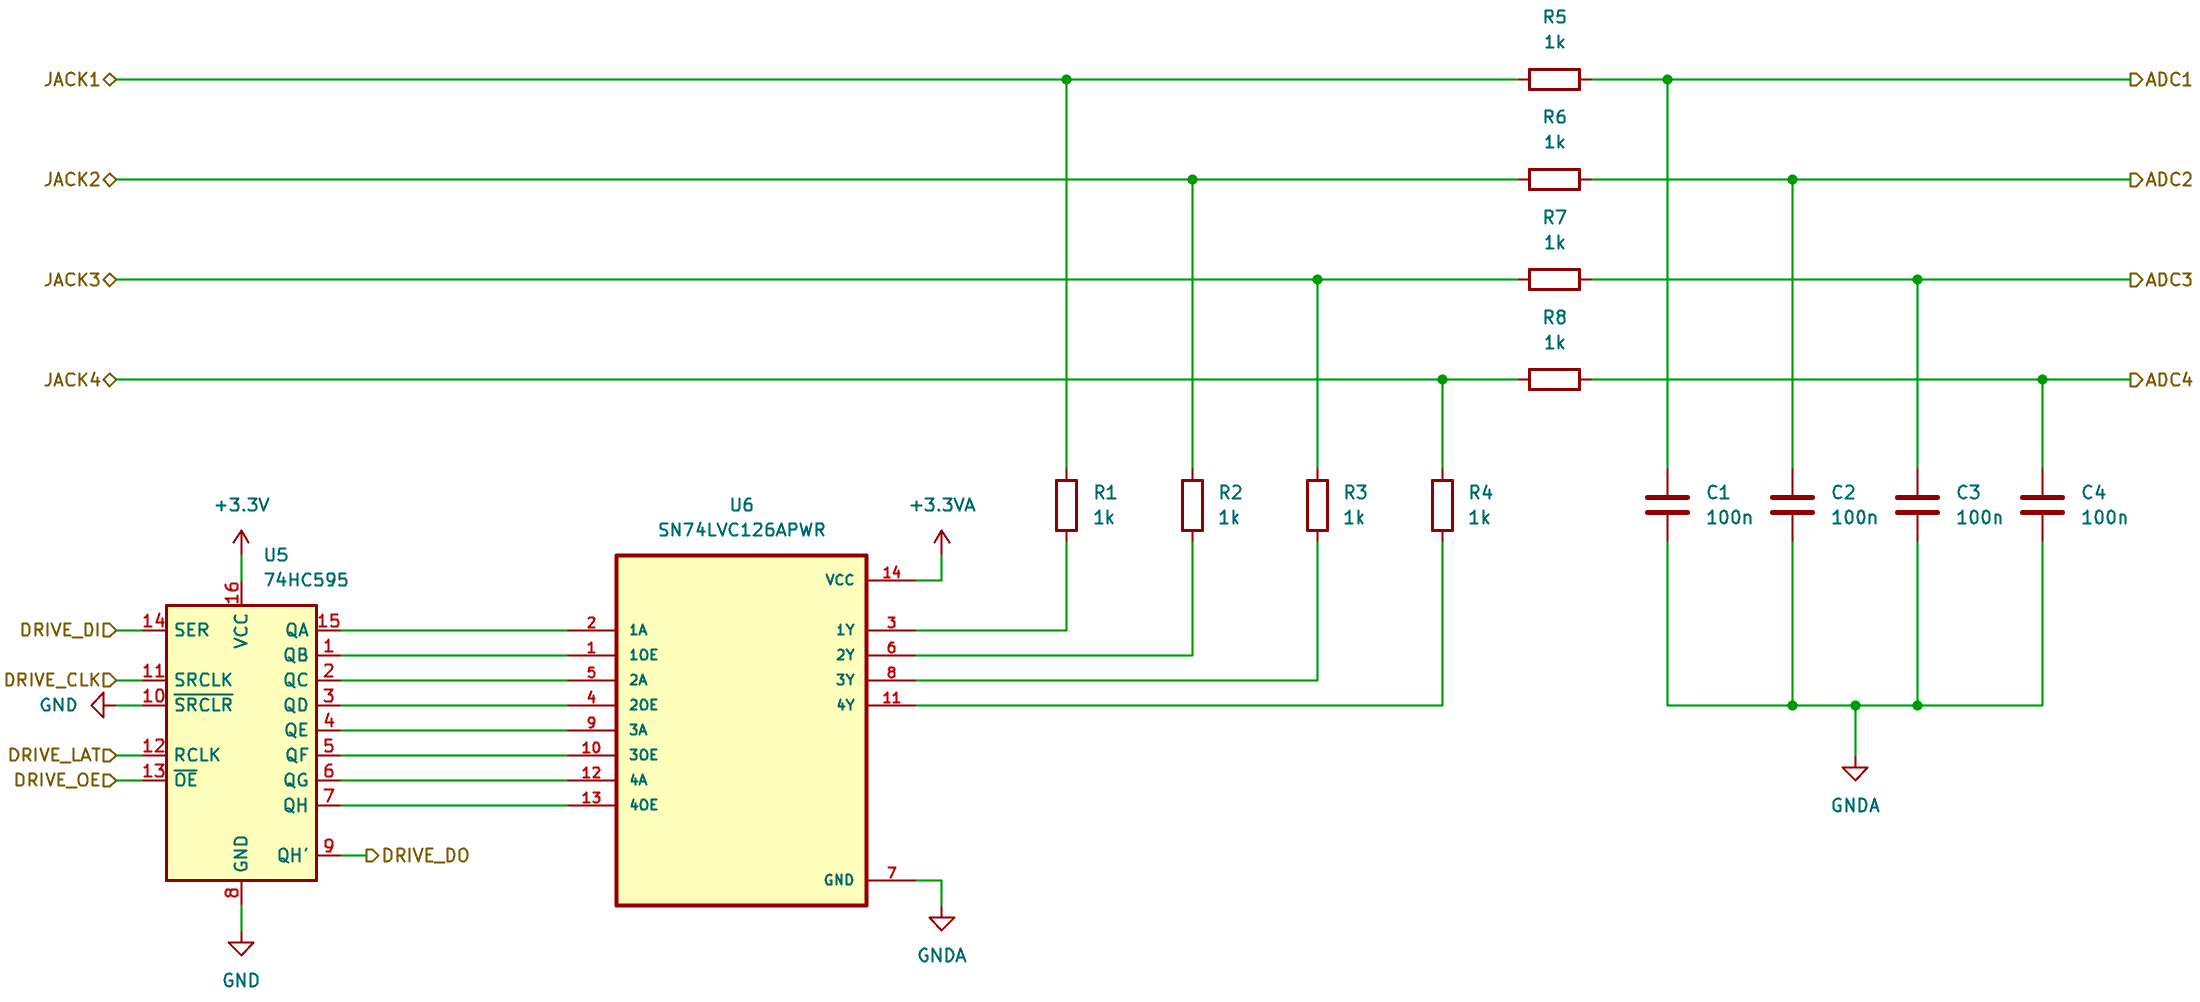
\includegraphics[width=0.85\linewidth]{04-implementation/figures/frontend-milestone-1}
    \caption{Milestone 1: Tristate Buffers}
    \label{fig:frontend-milestone-1}
  \end{subfigure}

  \vspace{4mm}
  \begin{subfigure}[t]{\linewidth}
    \centering
    \placeholderfigure[0.85\linewidth]{
      \textbf{Content.} The pull stage of one jack of the final board, cropped from \cref{fig:frontend-final}: U6 (74HC595), U15 and U19 (TMUX1511) with the shared resistors R50 and R54, without the RC filters.
      \textbf{Focus.} Same scale and orientation as (a), so that buffer and switch versions can be compared directly.
      \textbf{How to obtain.} Crop \code{04-implementation/figures/frontend-final.png} or export the sheet \code{hardware/AnalogQuadChannel.kicad\_sch} with \code{kicad-cli sch export svg}.
    }
    \caption{Final PCB: Analog Switches}
    \label{fig:frontend-switches}
  \end{subfigure}
  \titledcaption{Pull Stage Before and After the Change}{\scaffoldinline{(a): each 74HC595 output pair drives data and output enable of one SN74LVC126A buffer, whose output reaches the contact through a \qty{1}{\kilo\ohm} resistor (R1--R4); R5--R8 and C1--C4 form the old filter. (b): one switch per contact and rail, all switches of a rail sharing one \qty{0.1}{\percent} resistor.}}
  \label{fig:pull-stage-history}
\end{figure}

\subsection*{Pull Switching}

\scaffold{
  Proposal: SPDT analog switches \cite{ti2026ts5a23157}. Milestone~1 and breadboard: tristate buffers (SN74LVC126A \cite{ti2026sn74lvc126a}) driven by a 74HC595 chain, two control bits per contact (data and output enable), with a \qty{1}{\kilo\ohm} resistor at each output (\cref{fig:frontend-milestone-1}). Reason for the change to TMUX1511 switches \cite{ti2025tmux1511} (author's statement in the final presentation): the buffers worked in most cases, but their output impedance is only specified as a range and changed with the applied voltage, while the current computation of \cref{eq:currents} needs a precisely known pull resistance. The on-resistance of the switches, about \qty{2}{\ohm}, is negligible against the \qty{1}{\kilo\ohm} resistor, and \qty{0.1}{\percent} resistors make the pull resistance a known quantity. Add the consequence that comes for free: because the switches of one rail share one resistor, only one contact per rail can be driven at a time, which is exactly the one-high-one-low pattern of \cref{sec:pair-measurement}. Date of the change: 30~August~2026, which required a new schematic and a new layout.
}

\openquestion{Breadboard parts}{
  Which ADC and which buffer IC did the breadboard prototype use? The firmware drove an AD7718 from 6~August~2026, the parts list of the prototype names an ADS1241 and SN74LVC126A, and one development session refers to \enquote{74HC125-type} buffers. Also confirm the capacitance at each contact of the breadboard (the firmware inferred \qtyrange{68}{100}{\nano\farad} from a measured time constant).
}

\subsection*{Analog-to-Digital Converter}

\scaffold{
  Proposal: ADS8688, a 16-bit SAR ADC with eight channels and input protection \cite{ti2026ads8688}. Milestone~1: AD7124-8, a 24-bit sigma-delta ADC that works from \qty{3.3}{\volt} and needs little external circuitry \cite{adi2026ad7124}. The prototype parts list then names the ADS1241 \cite{ti2026ads1241}, and the final board uses two AD7718 \cite{adi2001ad7718}. Reasons recorded in the concept notes: the AD7124-8 exists only in a \qtyproduct{5 x 5}{\milli\metre} 32-lead LFCSP, hard to solder by hand, and was not available in single quantities; the ADS1241 is available in SSOP but reaches only 15 samples per second (30 with a faster crystal) \cite{ti2026ads1241}, too slow once several contacts are multiplexed; the AD7718 comes in SOIC-28 and converts at up to \qty{1365}{\hertz} with chopping disabled \cite{adi2001ad7718}. Name the price paid: two ADCs, each with its own \qty{32.768}{\kilo\hertz} crystal, and an input range of \qty{2.56}{\volt} that forced the analog rail down to \qty{2.5}{\volt} (next paragraph).
}

\openquestion{Reason for the AD7718}{
  The reasons above come from an early concept chat, not from the author. Confirm them or state the actual reason (availability, package, price, speed) for leaving the AD7124-8, and whether the ADS1241 was ever built up.
}

\subsection*{Analog Rail and Reference}

\scaffold{
  Milestone~1 planned an analog \qty{3.3}{\volt} rail. The final board pulls up to a \qty{2.5}{\volt} LDO rail that is at the same time the reference input of both ADCs, which makes every reading ratiometric: a shift of the rail moves the measured voltages and the reference together. Reason: the input range of the AD7718 ends at \qty{2.56}{\volt} with a \qty{2.5}{\volt} reference \cite{adi2001ad7718}. Call the rail a rail, not a precision reference: it is an ADP7142 LDO \cite{adi2025adp7142}.
}

\subsection*{Supply Split and Grounding}

\scaffold{
  Proposal and milestone~1 planned a separate analog supply and an analog ground joined to the digital ground at a single star point near the ADC \cite{benson2026proposal, kester2009mt031}. The final board has one \qty{3.3}{\volt} rail (named \net{+3.3VA}) for the ADCs' analog and digital supply, the shift registers and the switches, and one ground net poured on both layers of the two-layer board. State the reason in one or two sentences.
}

\openquestion{Reason for one ground net}{
  The decision to drop the star point and the separate analog supply is described as deliberate, but its reason is not recorded. Give it (for example: a sigma-delta ADC with low input bandwidth, short distances, a continuous ground plane on a two-layer board being the safer choice).
}

\subsection*{Input Filter}

\scaffold{
  Milestone~1: \qty{1}{\kilo\ohm} and \qty{100}{\nano\farad} per input; final board: \qty{10}{\kilo\ohm} and \qty{10}{\nano\farad}, corner frequency \qty{1.6}{\kilo\hertz}. Give the reason. Arguments available from the development notes: the corner stays the same order of magnitude while the capacitor that floating contacts must charge is ten times smaller (settling, \cref{sec:analog-front-end}); the filter still attenuates the region around the \qty{32.768}{\kilo\hertz} modulator clock of the AD7718 by about a factor of 20 and protects against RF pickup on long cables and ESD.
}

\openquestion{Reason for the filter values}{
  Why did the input filter change from \qty{1}{\kilo\ohm}/\qty{100}{\nano\farad} to \qty{10}{\kilo\ohm}/\qty{10}{\nano\farad}? The arguments in the box above were written after the board was ordered.
}

\subsection*{Contacts per Jack}

\scaffold{
  Milestone~1 switched four contacts per jack with one unused. Reason (final presentation): the switch and buffer ICs have four channels, so the fourth channel was free; it was connected to the tip switch of the jack and became the plug detection of \cref{sec:plug-detection}.
}

\subsection*{Microcontroller}

\scaffold{
  Proposal: STM32G4 or RP2040, both with native USB. Milestone~1 and later: the Raspberry Pi Pico~2 module \cite{rpi2026pico2w}; arguments from the milestone notes and the final presentation: a bare chip would need USB, crystal and flash added by hand, while the module is tested hardware; an STM32 has a faster CPU but needs more external parts and a proprietary USB stack; the Pico offers simple debugging through a debug probe, USB MIDI, two SPI peripherals (one for the ADCs, one for the shift registers) and, in the W variant, WiFi for a test interface.
}

\subsection*{Input Protection}

\scaffold{
  Milestone~1 used an ideal-diode controller (LM74700) for reverse-polarity protection. It was replaced by a passive P-channel MOSFET because the controller targets battery and automotive rails rather than a DC input from a wall adapter, which the author called a mistake of the first design. The final chain is a resettable fuse, a bidirectional TVS diode and the P-MOSFET with a gate Zener (details in \cref{sec:microcontroller-power}).
}

\openquestion{Supply voltage and polarity}{
  Which input voltage is the board designed for (an early session assumed \qty{9}{\volt}, the \qty{15}{\volt} clamp parts suggest up to \qty{12}{\volt}), and is reverse polarity blocked or made to work? The final schematic has no rectifier bridge.
}

% !TEX root = ../main.tex

\section{Analog Front End}
\label{sec:analog-front-end}

\scaffold{
  \textbf{Paragraph 1, the circuit.} Link: \cref{sec:design-history} explained why switches replaced the buffers. Walk through \cref{fig:frontend-final} for one jack, in the order the control signal passes: the 74HC595 \cite{ti2026sn74hc595} (U6) receives the drive pattern over SPI and latches it; its outputs select the switches of U15, which connect a contact to R50 (\qty{1}{\kilo\ohm}, \qty{0.1}{\percent}) and the \qty{2.5}{\volt} rail, and of U19, which connect it to R54 and ground. Each contact reaches its ADC input through R15--R18 (\qty{10}{\kilo\ohm}) with C23--C26 (\qty{10}{\nano\farad}) to ground. The four shift registers form one chain from the microcontroller to the fourth jack; their output enable is pulled high, so all switches stay open until the firmware writes the first pattern. Mention that the drive enum in the firmware makes it impossible to close the pull-up and pull-down switch of one contact at the same time.
}

\begin{figure}[htbp]
  \centering
  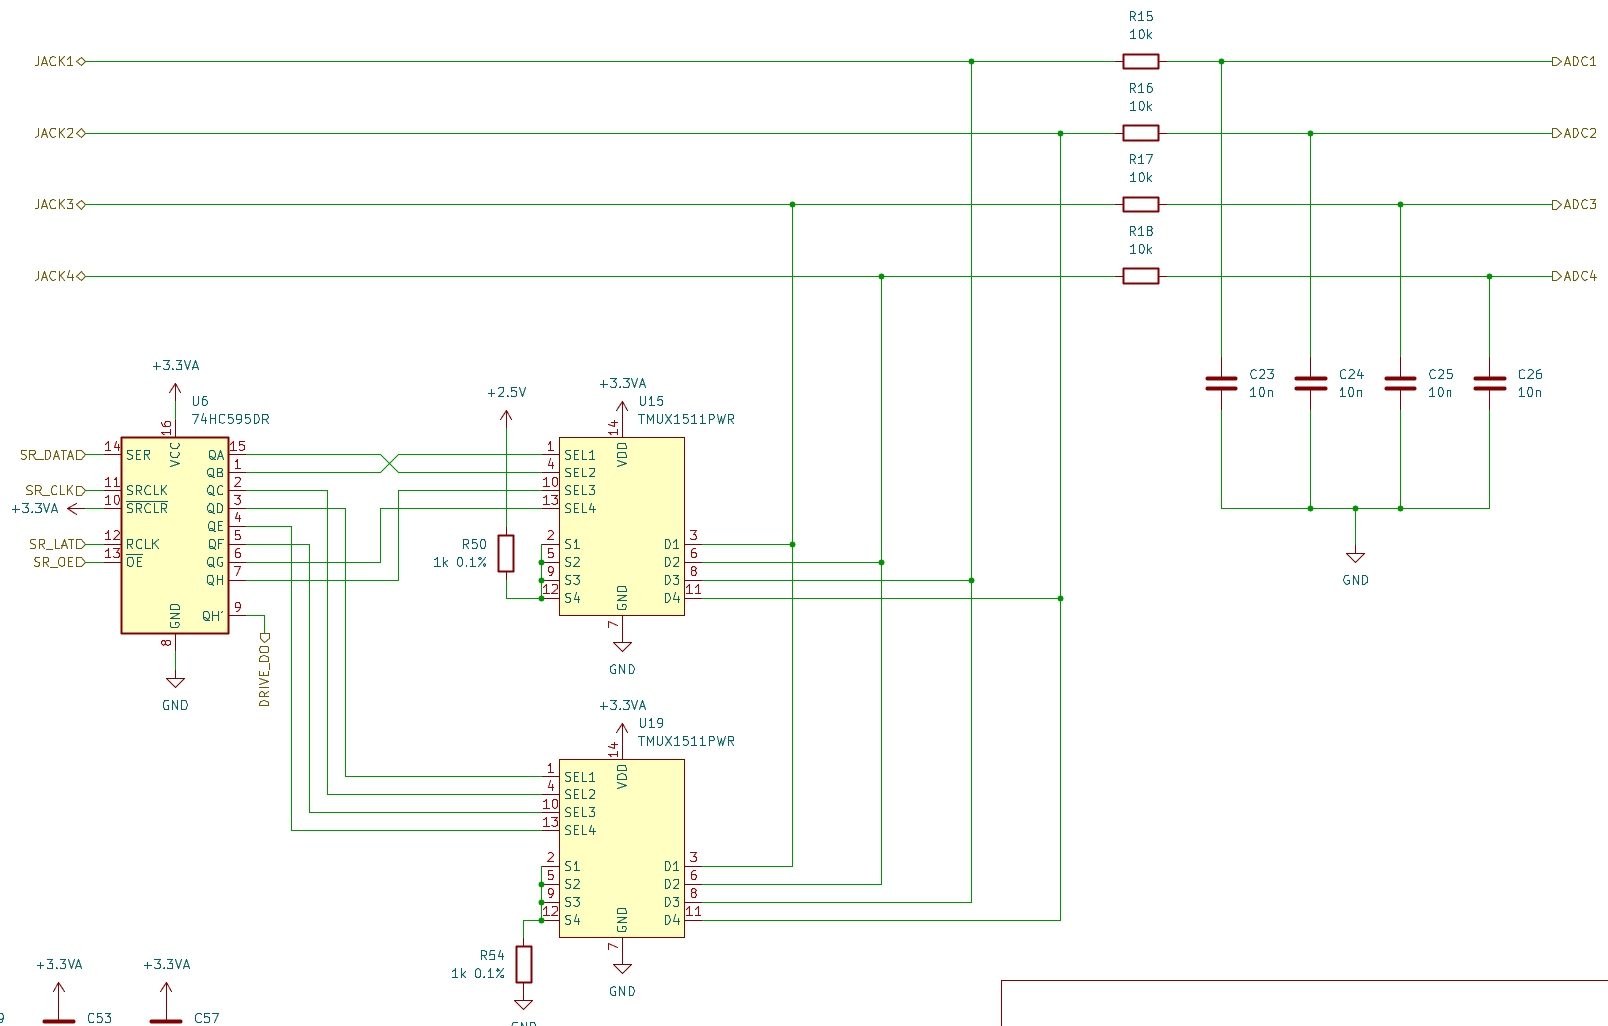
\includegraphics[width=\linewidth]{04-implementation/figures/frontend-final}
  \titledcaption{Analog Front End of One Jack}{\scaffoldinline{Name U6, U15, U19, R50, R54, R15--R18 and C23--C26 and their role; explain that JACK1--JACK4 are the four contacts of one jack (tip, ring, sleeve, tip switch, check the order against \code{src/board.rs}) and ADC1--ADC4 their ADC inputs. Source: KiCad sheet \code{hardware/AnalogQuadChannel.kicad\_sch}.}}
  \label{fig:frontend-final}
\end{figure}

\scaffold{
  \textbf{Paragraph 2, settling.} When the drive pattern changes, a floating contact charges the filter capacitor through the pedal and the filter resistor. Present \cref{eq:settling}: the firmware waits two time constants, between \qty{1}{\milli\second} and \qty{400}{\milli\second}, with $R_\mathrm{net}$ the resistance of the network through which the floating contact charges, known from the previous solve (an unknown network is assumed to be \qty{100}{\kilo\ohm}). Compute $\tau$ for a \qty{10}{\kilo\ohm} pedal (about \qty{0.2}{\milli\second}) and a \qty{500}{\kilo\ohm} pedal (about \qty{5}{\milli\second}). Refer to \cref{sec:results-settling} for the measured time constant.
}

\begin{equation}
  t_\mathrm{settle} = 2\,\tau,
  \qquad
  \tau = \bigl(R_\mathrm{net} + R_\mathrm{f}\bigr)\,C_\mathrm{f},
  \qquad
  \qty{1}{\milli\second} \leq t_\mathrm{settle} \leq \qty{400}{\milli\second}
  \label{eq:settling}
\end{equation}

\scaffold{
  \textbf{Paragraph 3, choice of the pull resistance.} The pull resistance trades position resolution against current resolution: across a pedal of resistance $R$ lies $U\,R/(R + 2R_\mathrm{p})$, across each pull resistor $U\,R_\mathrm{p}/(R + 2R_\mathrm{p})$. Present \cref{tab:pull-resistance} and draw the conclusion: the position uses the span and is fine with any value; only the total resistance of high-value pedals depends on the drop. With \qty{1}{\kilo\ohm} and \qty{0.4}{\milli\volt} noise every pedal up to about \qty{500}{\kilo\ohm} still resolves; \qty{4.7}{\kilo\ohm} would be the value to fit if accurate totals of 250 to \qty{500}{\kilo\ohm} pedals mattered (\cref{ch:conclusion}).
}

\begin{table}[htbp]
  \centering
  \titledcaption{Voltage Span and Pull Drop}{\scaffoldinline{Explain that each cell gives the voltage across the pedal and the drop across one pull resistor for a \qty{2.5}{\volt} rail; the fitted value is \qty{1}{\kilo\ohm}. Source: \code{docs/fast-tracking.md}.}}
  \label{tab:pull-resistance}
  \begin{tabular}{@{}l *{3}{c}@{}}
    \toprule
    \textbf{Pull resistance} & \textbf{\qty{10}{\kilo\ohm} pedal} & \textbf{\qty{100}{\kilo\ohm} pedal} & \textbf{\qty{500}{\kilo\ohm} pedal} \\
    \midrule
    \qty{1}{\kilo\ohm} (fitted) & \qty{2.08}{\volt} / \qty{208}{\milli\volt} & \qty{2.45}{\volt} / \qty{24}{\milli\volt} & \qty{2.49}{\volt} / \qty{5}{\milli\volt} \\
    \qty{2.2}{\kilo\ohm} & \qty{1.74}{\volt} / \qty{382}{\milli\volt} & \qty{2.40}{\volt} / \qty{53}{\milli\volt} & \qty{2.48}{\volt} / \qty{11}{\milli\volt} \\
    \qty{4.7}{\kilo\ohm} & \qty{1.29}{\volt} / \qty{606}{\milli\volt} & \qty{2.29}{\volt} / \qty{107}{\milli\volt} & \qty{2.45}{\volt} / \qty{23}{\milli\volt} \\
    \qty{10}{\kilo\ohm} & \qty{0.83}{\volt} / \qty{833}{\milli\volt} & \qty{2.08}{\volt} / \qty{208}{\milli\volt} & \qty{2.45}{\volt} / \qty{49}{\milli\volt} \\
    \bottomrule
  \end{tabular}
\end{table}

\openquestion{Choice of 1 kOhm}{
  Was \qty{1}{\kilo\ohm} chosen with the analysis of \cref{tab:pull-resistance} in mind, or was the analysis done afterwards on the finished board? The answer decides whether paragraph~3 describes a design decision or a later evaluation.
}

% !TEX root = ../main.tex

\section{Analog-to-Digital Conversion}
\label{sec:conversion}

\scaffold{
  \textbf{Paragraph 1, the ADCs.} Two AD7718 \cite{adi2001ad7718} read the 16 contacts (\cref{fig:adc}): U4 the two jacks on the left of the PCB, U5 the two on the right; the case order of the firmware numbers the jacks from J5 to J2 because the PCB is mounted upside down. Each ADC runs in ten-channel pseudo-differential mode against AINCOM at ground, since the second jack on each chip uses AIN9, which doubles as a reference input in the eight-channel mode. AIN6 is tied to ground and AIN10 to the \qty{2.5}{\volt} rail on both chips, which gives a self-test of the whole conversion path (\cref{sec:results-self-test}). Each chip has its own \qty{32.768}{\kilo\hertz} crystal (Y1, Y2) with \qty{18}{\pico\farad} load capacitors. Both share SPI0 at \qty{4}{\mega\hertz} with separate chip-select and ready lines.
}

\begin{figure}[htbp]
  \centering
  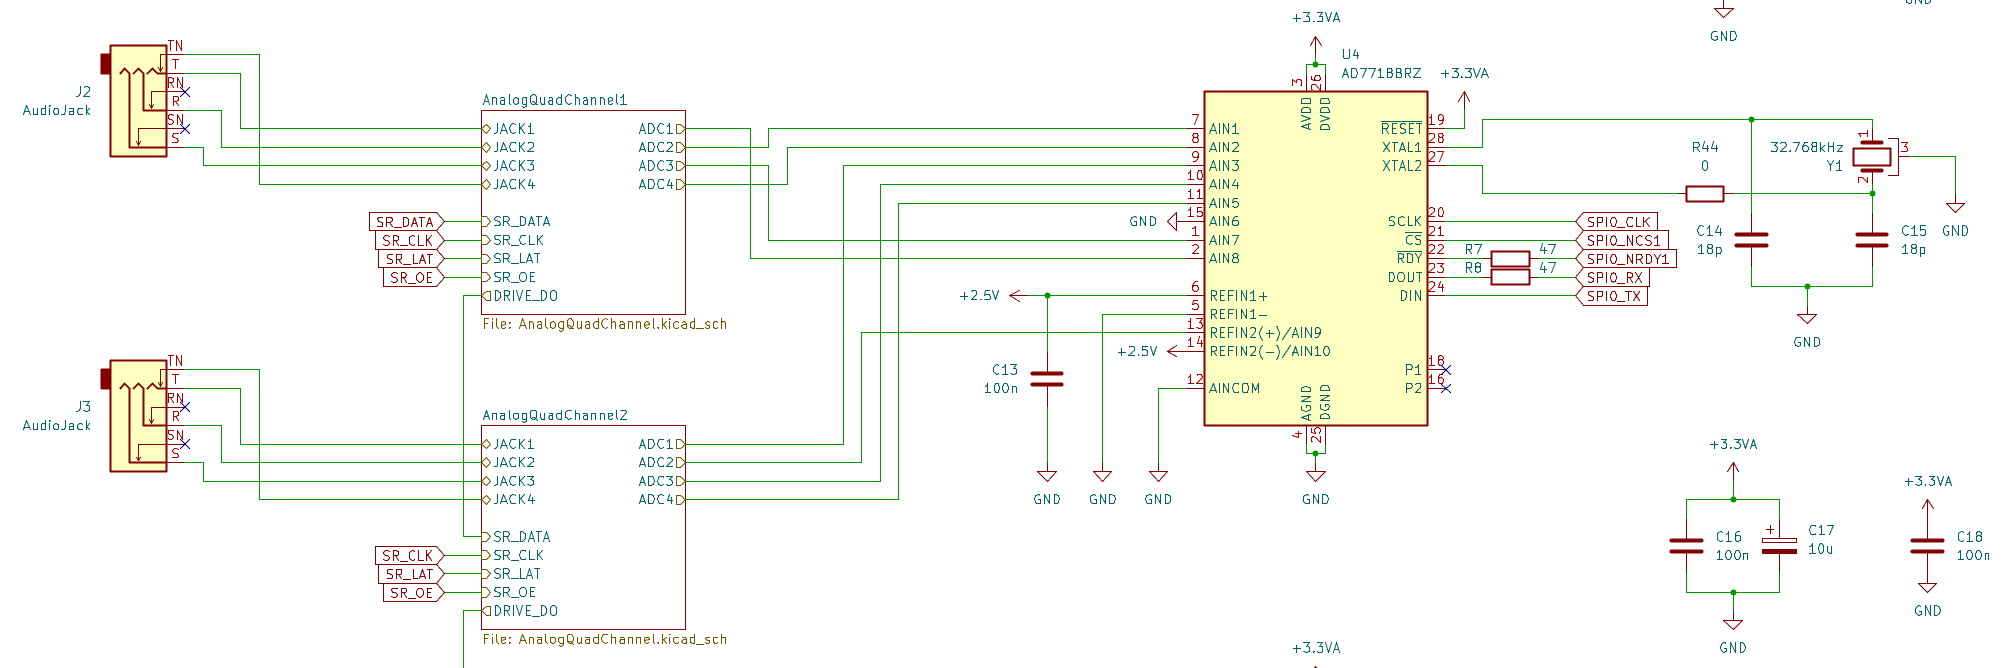
\includegraphics[width=\linewidth]{04-implementation/figures/adc}
  \titledcaption{ADCs}{\scaffoldinline{Name U4 and U5, the crystals, the reference connection to the \qty{2.5}{\volt} rail, the self-test inputs AIN6 and AIN10, and the SPI and ready signals to the microcontroller. Source: KiCad sheet \code{hardware/AnalogFrontend.kicad\_sch}; enlarge or split if the labels are not readable at text width.}}
  \label{fig:adc}
\end{figure}

\scaffold{
  \textbf{Paragraph 2, the filter and its settling.} The AD7718 is a sigma-delta ADC with a sinc\textsuperscript{3} decimation filter \cite{adi2001ad7718}. With chopping disabled, which the firmware uses for channel throughput, the output rate is programmable from \qty{16.06}{\hertz} to \qty{1365.33}{\hertz}; a channel change counts as a synchronized step and needs three conversion periods to settle \cite{adi2001ad7718}. Explain the consequence that shapes the whole firmware: every reading that changes the channel costs three conversion periods, independent of how fast the analog input settles. Mention that the datasheet requires recalibration after gain or temperature changes in this mode, and that the firmware calibrates once at start-up and measures its own rails (\cref{sec:pair-measurement}).
}

\scaffold{
  \textbf{Paragraph 3, the SPI interface.} Every SPI and shift-register line has a \qty{47}{\ohm} series resistor at its driver to slow the edges and damp reflections on the two-layer board. A chip-select guard of \qty{10}{\micro\second} before and after every transfer was found sufficient on the PCB, where the breadboard needed \qty{50}{\micro\second} and showed outlying codes otherwise; the firmware skips the control-register write when the channel does not change. Two driver bugs found on the breadboard are worth one sentence each: the ready line was polled before the chip had registered the conversion command, which corrupted the calibration, and toggling chip select too quickly made the chip lose synchronization.
}

\openquestion{Choice of 47 Ohm}{
  A design session recommended \qtyrange{22}{33}{\ohm}; the board has \qty{47}{\ohm}. Give the reason for the value.
}

% !TEX root = ../main.tex

\section{Microcontroller and Power Supply}
\label{sec:microcontroller-power}

\scaffold{
  \textbf{Paragraph 1, microcontroller.} The Raspberry Pi Pico~2~W module \cite{rpi2026pico2w} carries the RP2350 \cite{rpi2026rp2350} and a CYW43439 WiFi chip. Walk through \cref{fig:microcontroller}: SPI0 to the ADCs (clock GPIO18, TX GPIO19, RX GPIO16, chip selects GPIO17 and GPIO20, ready GPIO21 and GPIO22), SPI1 to the shift-register chain (clock GPIO14, data GPIO15, latch GPIO13, output enable GPIO11), and the LED data line on GPIO6 through a 74AHCT1G125 level shifter, since the WS2812B \cite{worldsemi2026ws2812b} expects a \qty{5}{\volt} logic level. The module's own \qty{3.3}{\volt} regulator is not connected to the board rail, and VBUS is unconnected.
}

\begin{figure}[htbp]
  \centering
  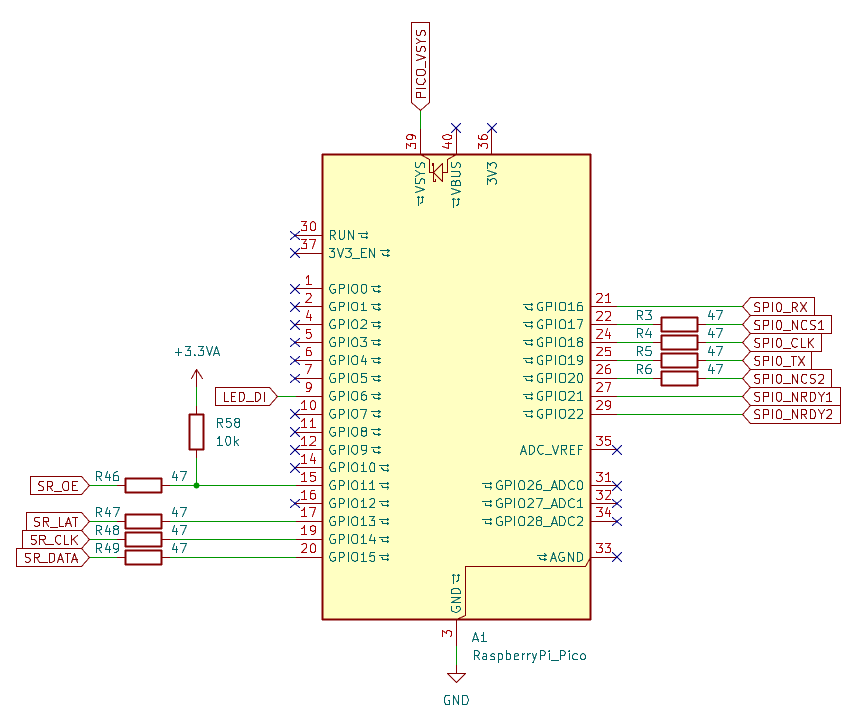
\includegraphics[width=0.75\linewidth]{04-implementation/figures/microcontroller}
  \titledcaption{Microcontroller}{\scaffoldinline{Name the two SPI buses, the \qty{47}{\ohm} series resistors R3--R6 and R46--R49, the LED data line and the unconnected supply pins. Source: KiCad sheet \code{hardware/Microcontroller.kicad\_sch}.}}
  \label{fig:microcontroller}
\end{figure}

\scaffold{
  \textbf{Paragraph 2, power input.} Walk through the left part of \cref{fig:power-supply}: barrel jack, resettable fuse MF-MSMF050-2 against overcurrent, bidirectional TVS diode SMBJ15CA against voltage spikes, and the P-channel MOSFET DMP3099L as reverse-polarity protection, its gate pulled to ground through \qty{100}{\kilo\ohm} and clamped by a \qty{15}{\volt} Zener diode. Give the reason for each part in a subordinate clause.
}

\scaffold{
  \textbf{Paragraph 3, rails.} Three ADP7142 LDOs \cite{adi2025adp7142} supply \qty{5}{\volt} (LEDs, level shifter and the Pico's VSYS through a Schottky diode that prevents back-feeding when the Pico's USB is connected), \qty{3.3}{\volt} (ADCs, shift registers, switches) and \qty{2.5}{\volt}. The \qty{2.5}{\volt} rail is cascaded from the \qty{3.3}{\volt} rail rather than from the input, so the reference sits behind two regulators. Solder jumpers JP1--JP3 between each LDO and its rail allow the current of every rail to be measured separately. One consequence for operation: the measurement rails derive only from the barrel jack, so USB alone powers only the microcontroller.
}

\scaffold{
  \textbf{Paragraph 4, LED power budget.} The \qty{5}{\volt} LDO delivers at most \qty{200}{\milli\ampere} \cite{adi2025adp7142} and is shared by the four LEDs and the Pico; four LEDs at full white would draw about \qty{240}{\milli\ampere}. The LED driver therefore scales every frame to at most 10 of 255 per color channel, about \qty{4}{\percent}, at the lowest driver level, so that no setting can exceed it.
}

\openquestion{LED limit}{
  The final presentation states a limit of about \qty{20}{\percent} (51 of 255); the firmware was later reduced to 10 of 255. Was the reduction made for the power budget, for visual brightness, or because of the WiFi tests? State the final value in the text.
}

\begin{figure}[htbp]
  \centering
  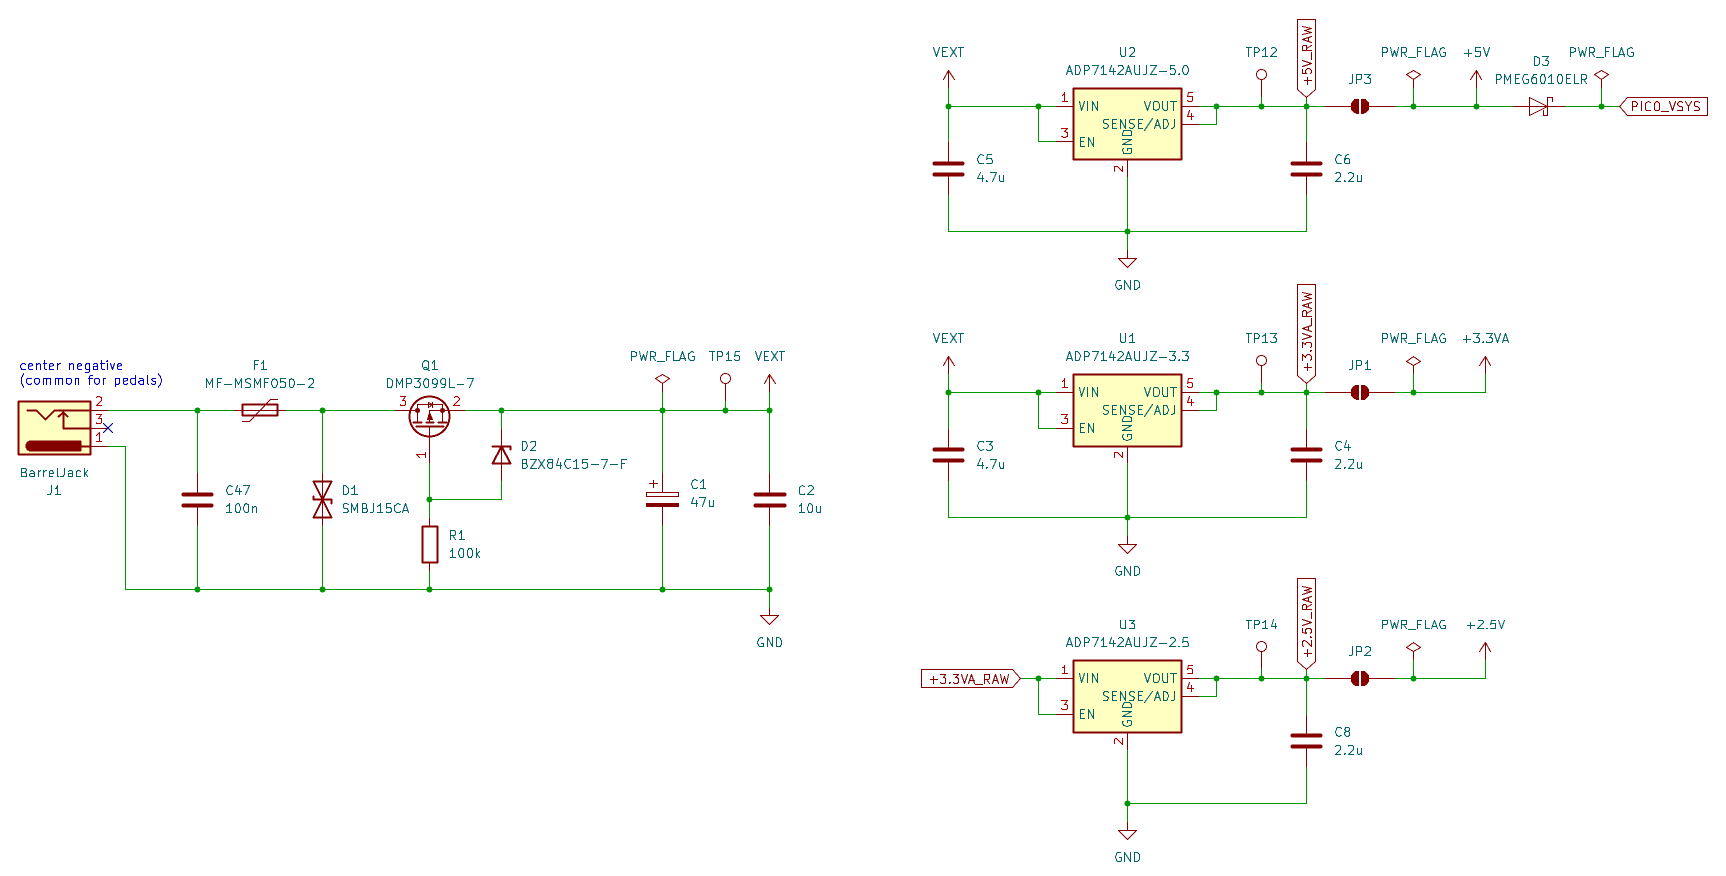
\includegraphics[width=\linewidth]{04-implementation/figures/power-supply}
  \titledcaption{Power Supply}{\scaffoldinline{Name the protection chain (F1, D1, Q1 with R1 and D2), the three LDOs U1--U3 with their output voltages, the cascade of U3 from the \qty{3.3}{\volt} rail, the solder jumpers JP1--JP3 and the Schottky diode D3. Source: KiCad sheet \code{hardware/Power.kicad\_sch}.}}
  \label{fig:power-supply}
\end{figure}

% !TEX root = ../main.tex

\section{PCB Layout and Assembly}
\label{sec:pcb}

\scaffold{
  \textbf{Paragraph 1, layout.} Describe \cref{fig:pcb-layout}: a two-layer board with 149 footprints, the four jacks along one edge, the jack blocks repeated four times, the power section with one copper fill per rail and the regulators between them. Ground is poured on both layers; the power input section has its own pour on the same net. 15 test points sit on the signals the measurements of \cref{ch:results} need: the shift-register lines (TP1--TP4), SPI0 with both chip selects and ready lines (TP5--TP11) and the four rails (TP12--TP15).
}

\begin{figure}[htbp]
  \centering
  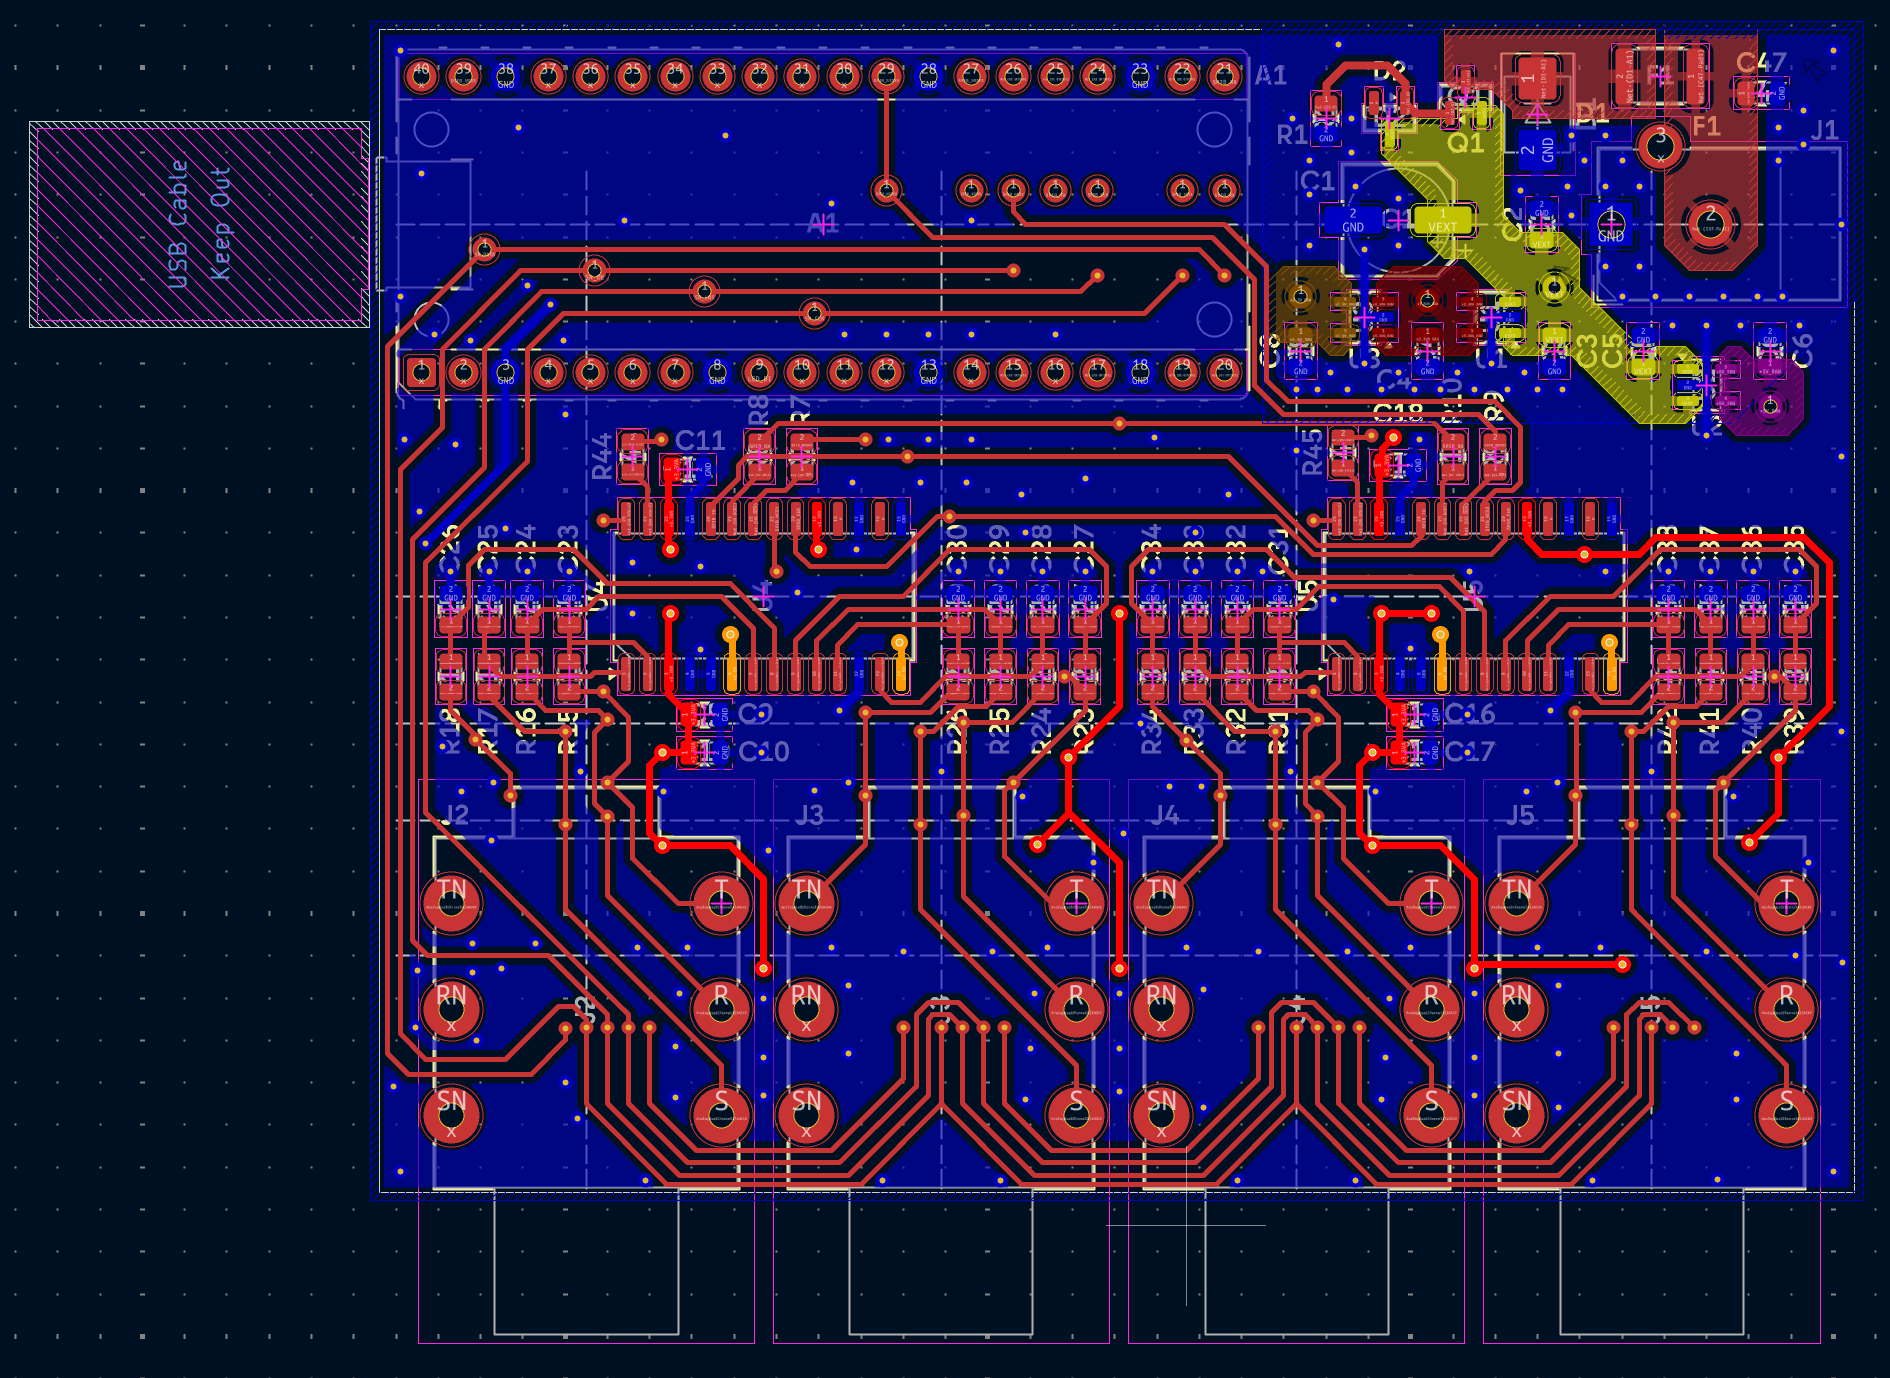
\includegraphics[width=0.85\linewidth]{04-implementation/figures/pcb-layout}
  \titledcaption{PCB Layout}{\scaffoldinline{Name the regions (jacks, four channel blocks, ADCs, microcontroller, power section) and the two copper layers shown. Source: KiCad \code{hardware/ExpressionController.kicad\_pcb}.}}
  \label{fig:pcb-layout}
\end{figure}

\scaffold{
  \textbf{Paragraph 2, assembly.} The top side was soldered by hand in separate blocks, the power supply first, and every rail was checked before the next block was populated; the bottom side was assembled with a stencil (first use for the author). The TMUX1511 in TSSOP-14 were the most difficult parts. Show \cref{fig:assembly}. The board-level self-test passed on its first run (\cref{sec:results-self-test}).
}

\begin{figure}[htbp]
  \centering
  \begin{subfigure}[t]{0.32\linewidth}
    \centering
    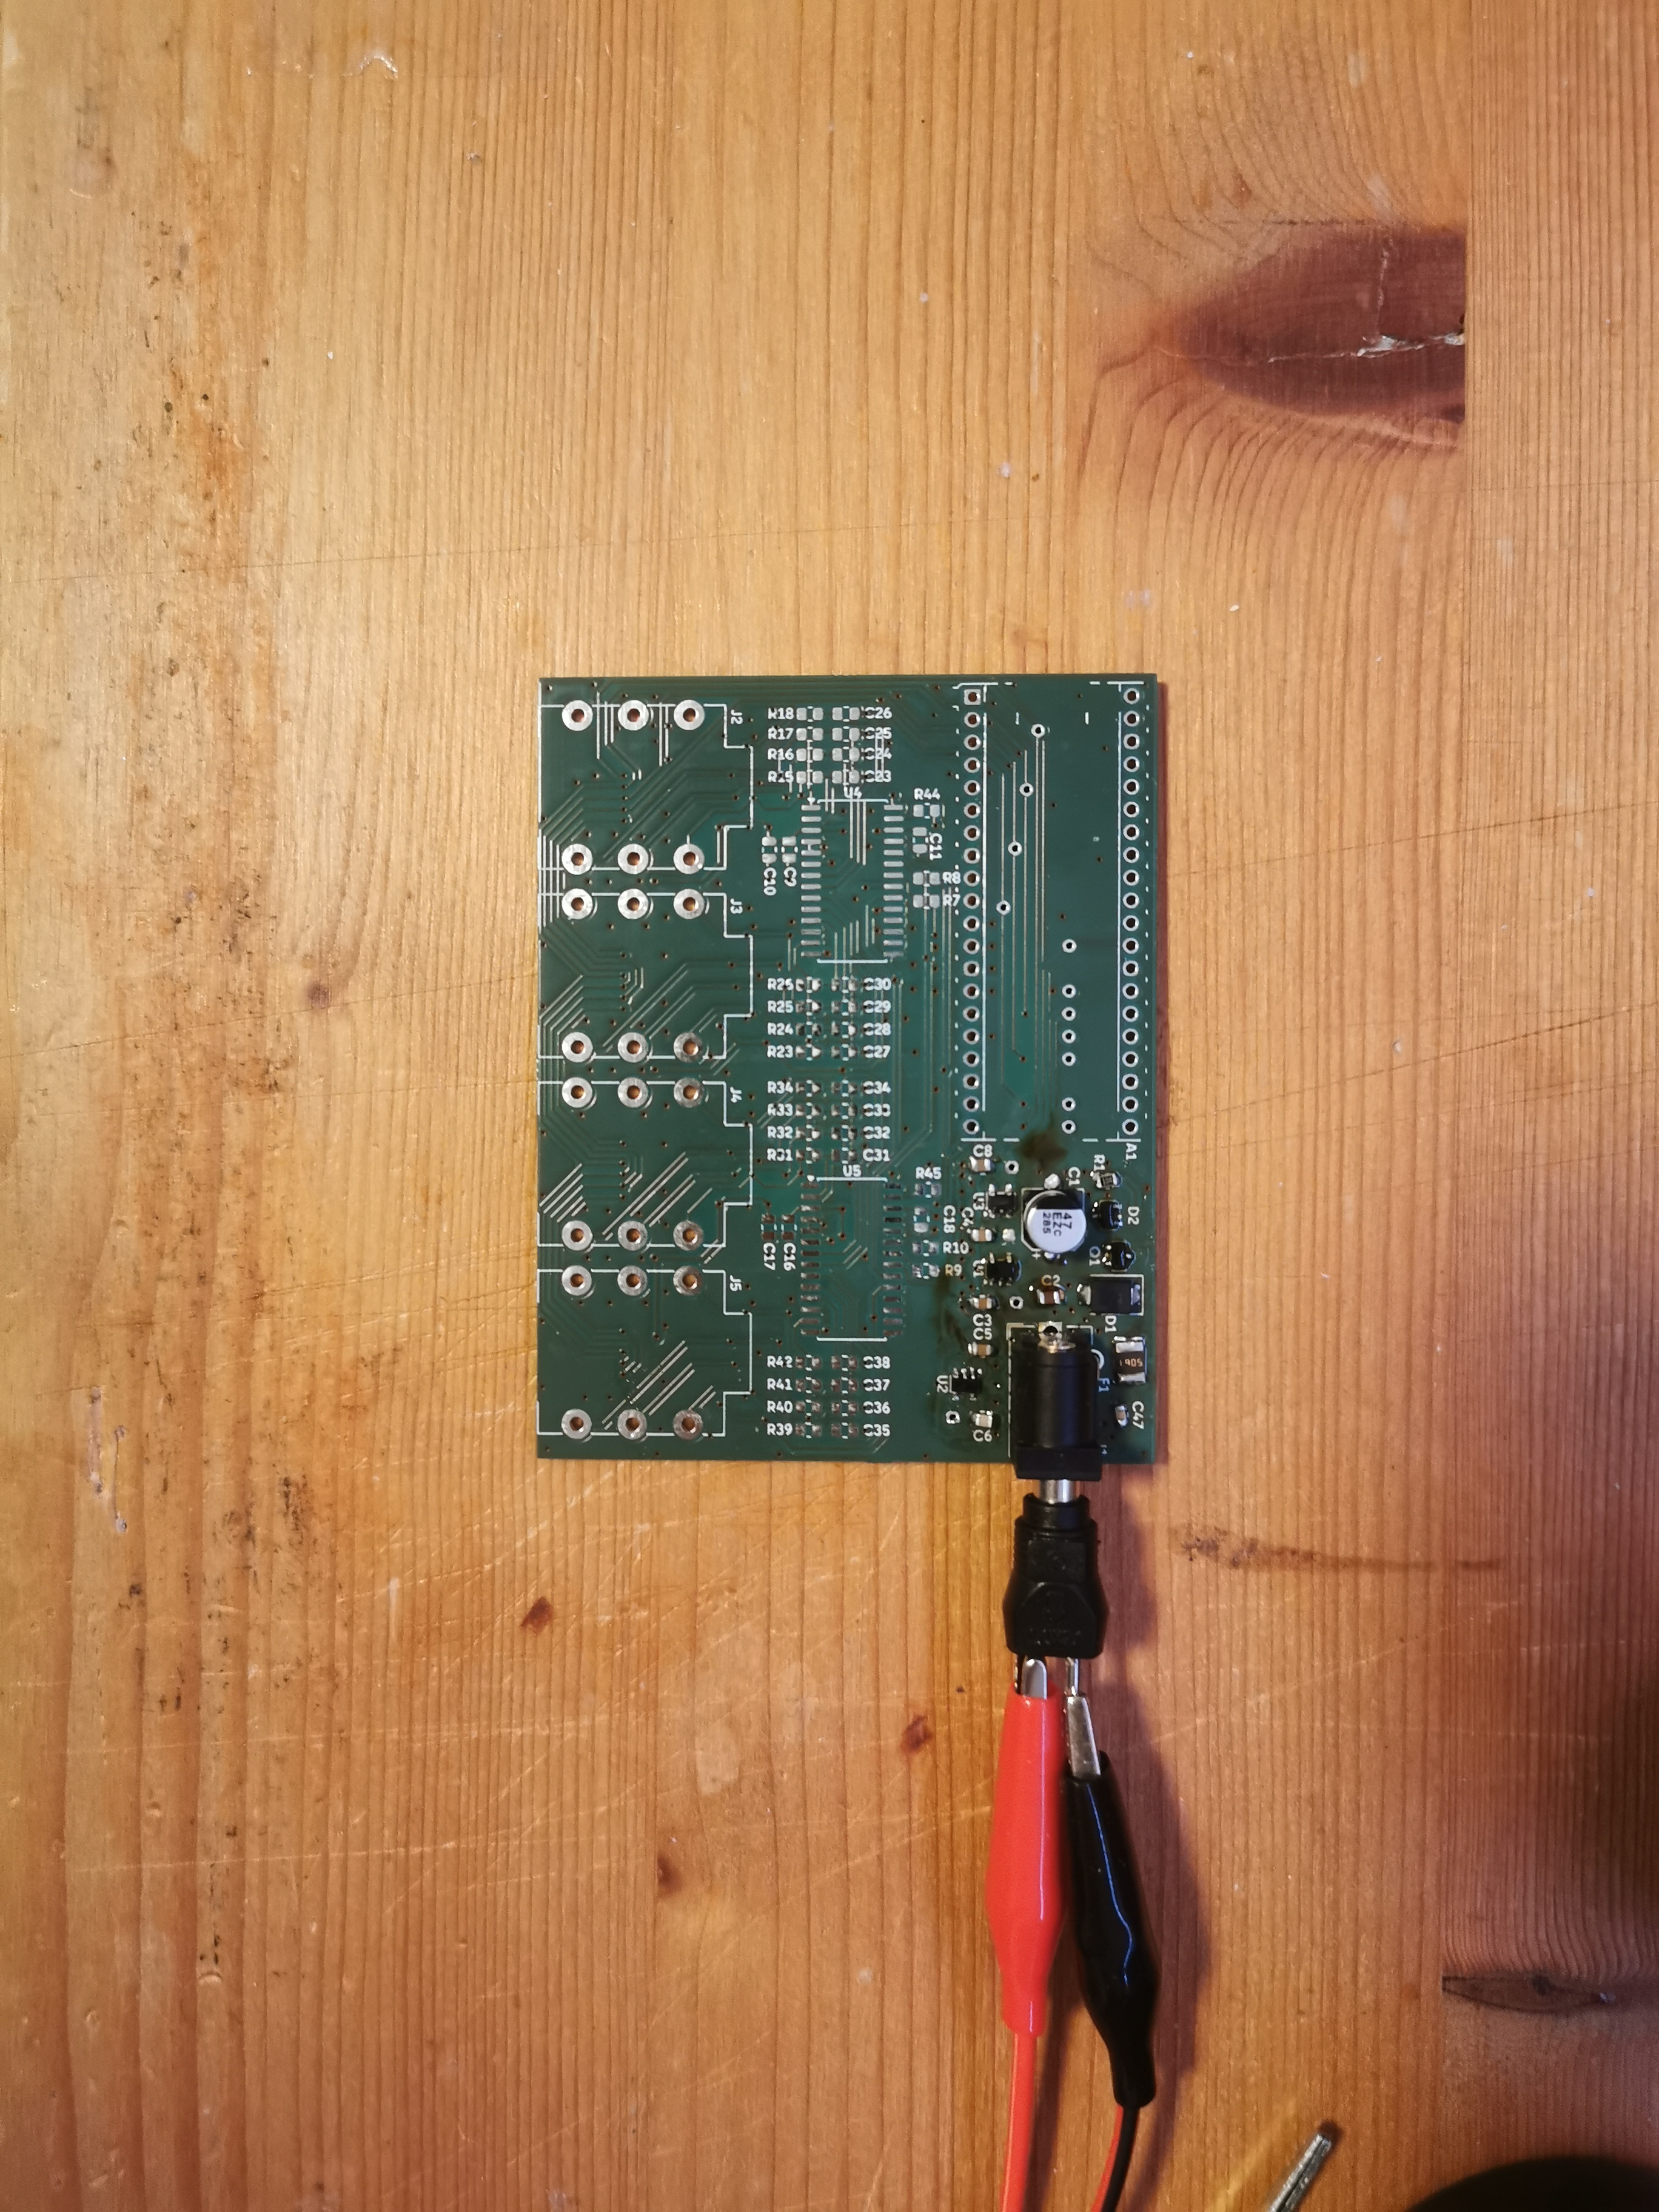
\includegraphics[width=\linewidth]{04-implementation/figures/assembly-top-side}
    \caption{Power Supply Populated}
    \label{fig:assembly-top-side}
  \end{subfigure}%
  \hfill%
  \begin{subfigure}[t]{0.64\linewidth}
    \centering
    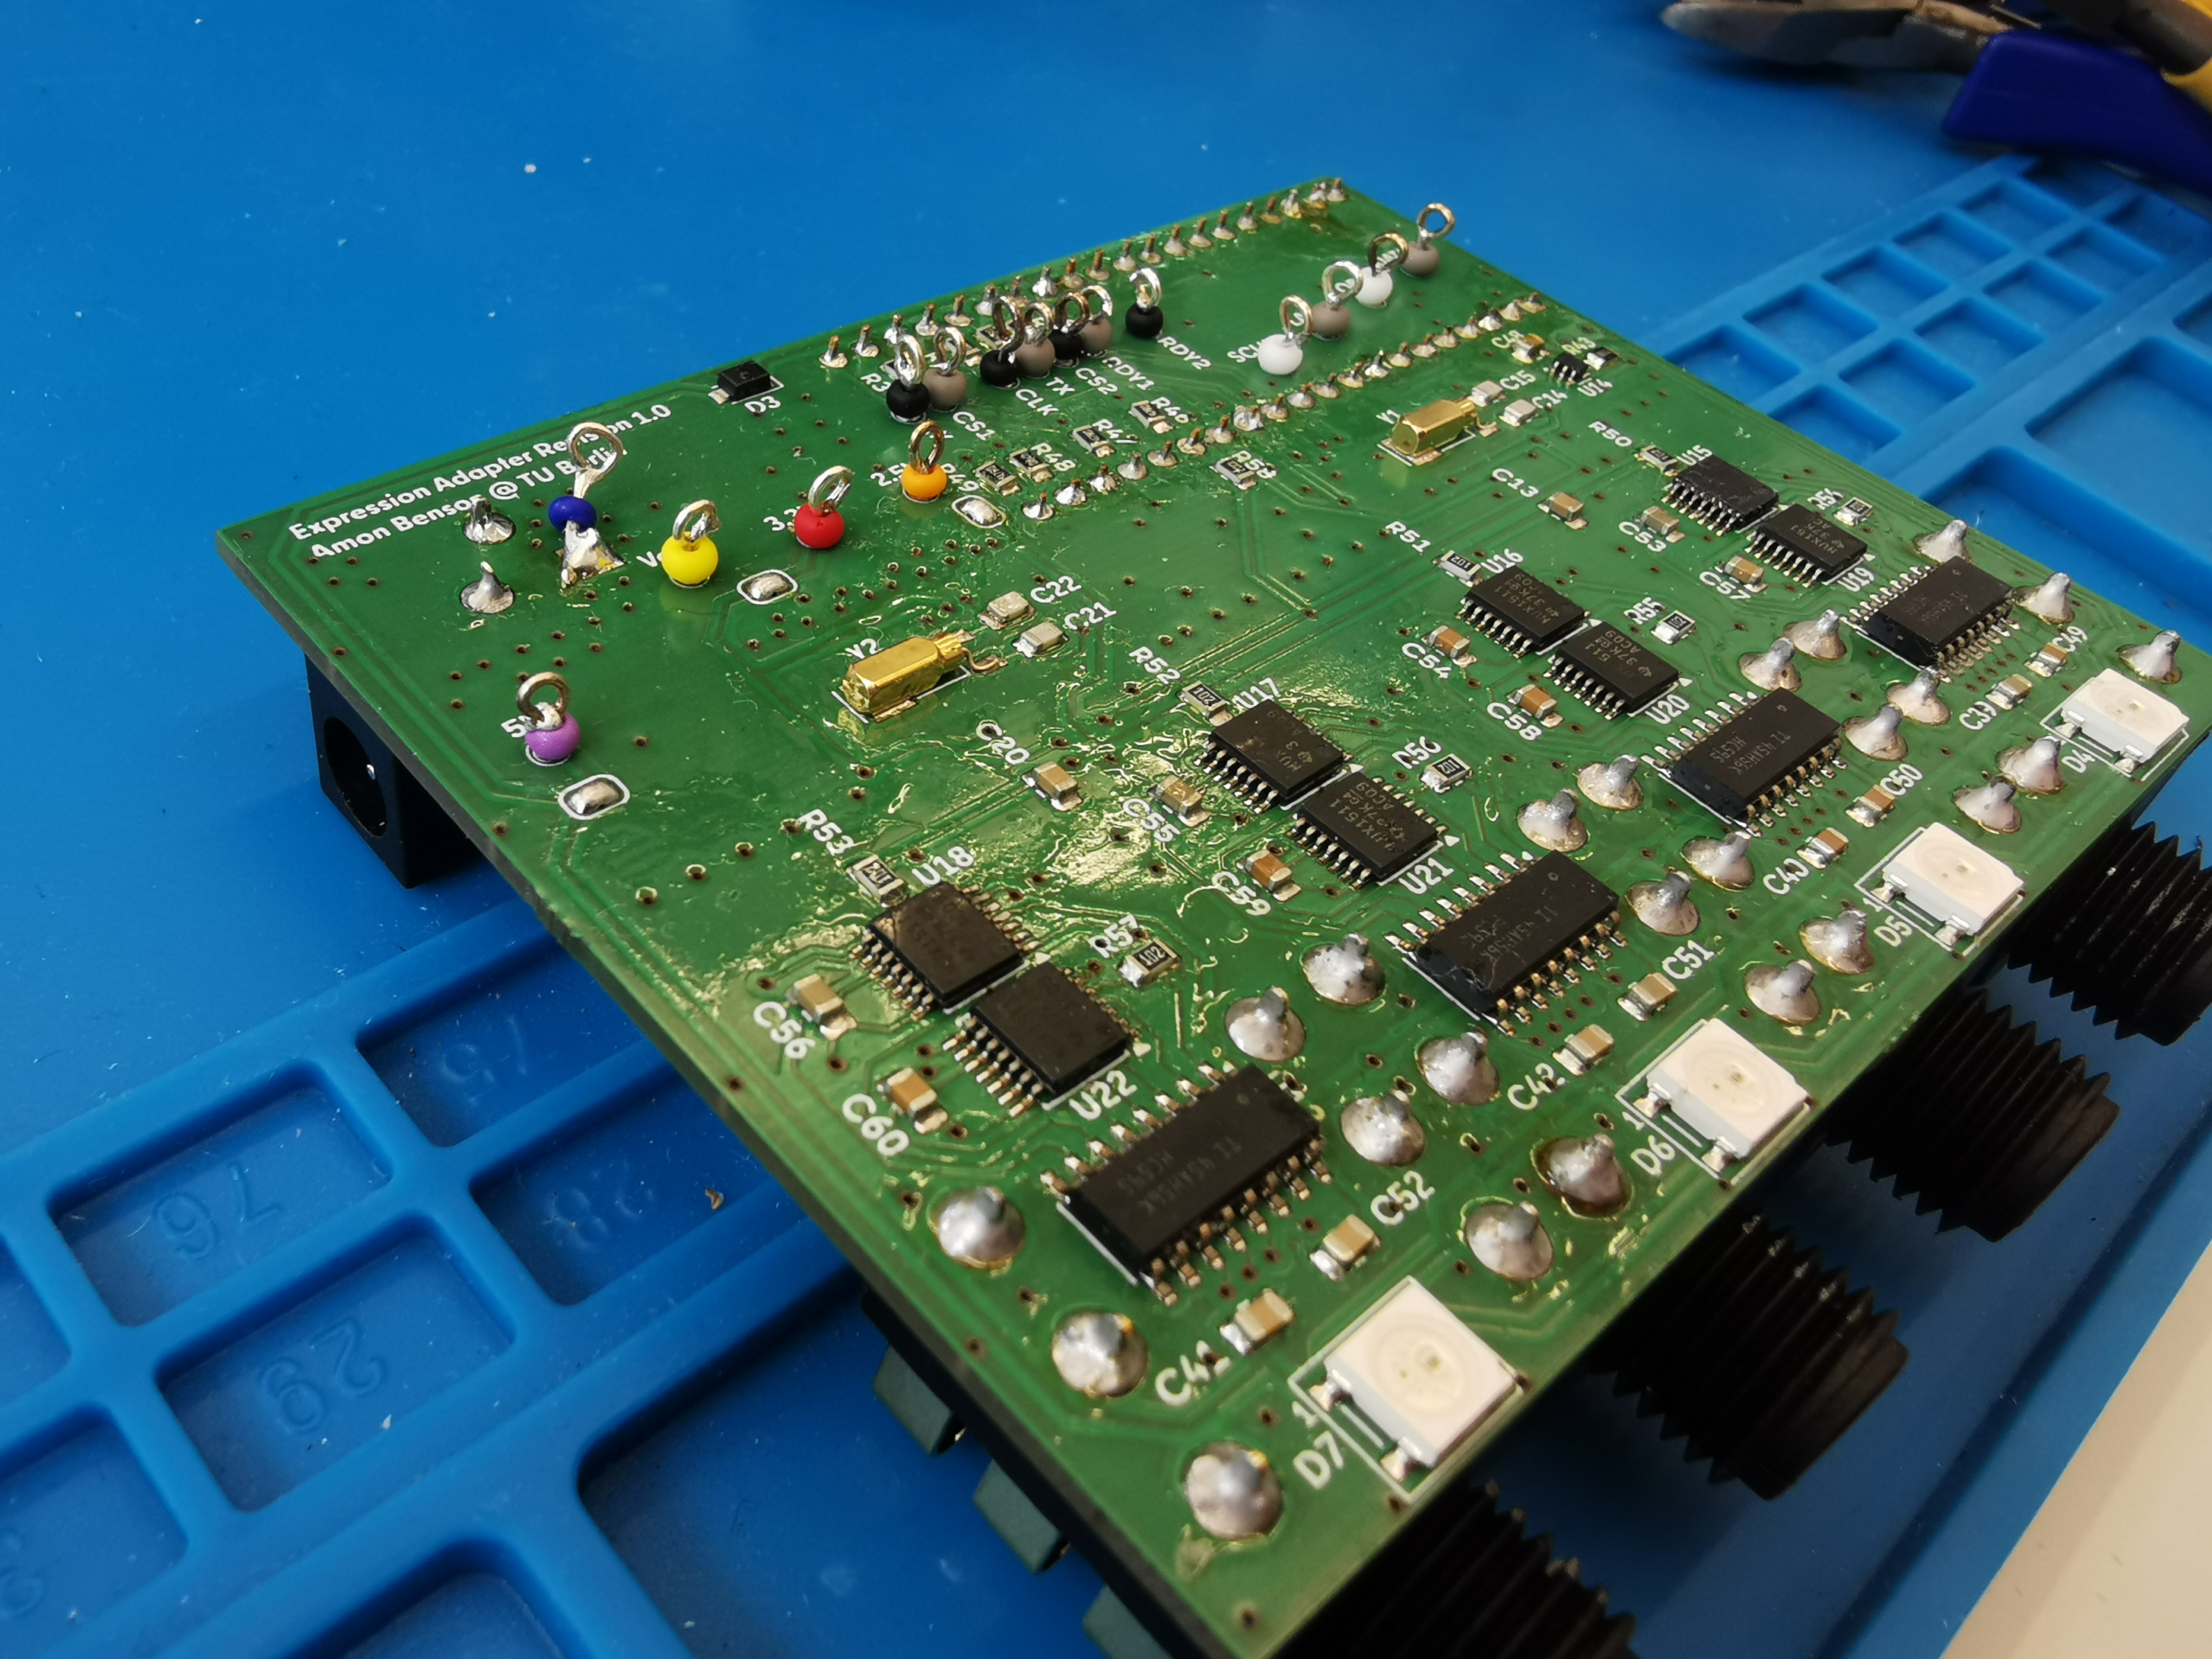
\includegraphics[width=\linewidth]{04-implementation/figures/assembly-complete}
    \caption{Assembled Board}
    \label{fig:assembly-complete}
  \end{subfigure}
  \titledcaption{PCB Assembly}{\scaffoldinline{(a) first assembly stage, check what is populated; (b) the assembled board with the switches, shift registers, ADCs and color-coded test points. Photos of the author; further photos in the folder \enquote{Final Images}.}}
  \label{fig:assembly}
\end{figure}

\openquestion{Board facts}{
  Give the board outline (about \qtyproduct{89 x 70}{\milli\metre} from the ground pour, not measured), the manufacturer of PCB and stencil, and the date the boards were ordered and arrived (git history: final assembly files 6~September, \enquote{after final fab order} 16~September, first firmware on the board 25~September~2026).
}

% !TEX root = ../main.tex

\section{Firmware Architecture}
\label{sec:firmware-architecture}

\scaffold{
  \textbf{Paragraph 1, language and framework.} The firmware is written in Rust \cite{rust2026} without the standard library and uses the asynchronous Embassy framework \cite{embassy2026} for the RP2350: drivers wait for interrupts as futures, so USB, WiFi, the LEDs and the measurement run as concurrent tasks on one core. The source is in the project repository \cite{benson2026expad}. One sentence on why this matters for the report: a stalled task cannot block the measurement, which became relevant for USB (\cref{sec:output}).
}

\scaffold{
  \textbf{Paragraph 2, two crates and their layers.} Walk through the layers: \code{board} is the only module that knows the PCB (pins, chips, which ADC channel reads which contact); the hardware abstraction layer drives chips (AD7718, shift registers and switches, LEDs, USB, WiFi) without knowing jacks; the scanner runs the measurement on the hardware; the separate library \code{expad-topology} holds the solver arithmetic of \cref{ch:measurement-principle} and the per-jack state machine and knows neither board nor chips. Present \cref{fig:firmware-overview} as the overview of the state machine's four stages and the output.
}

\begin{figure}[htbp]
  \centering
  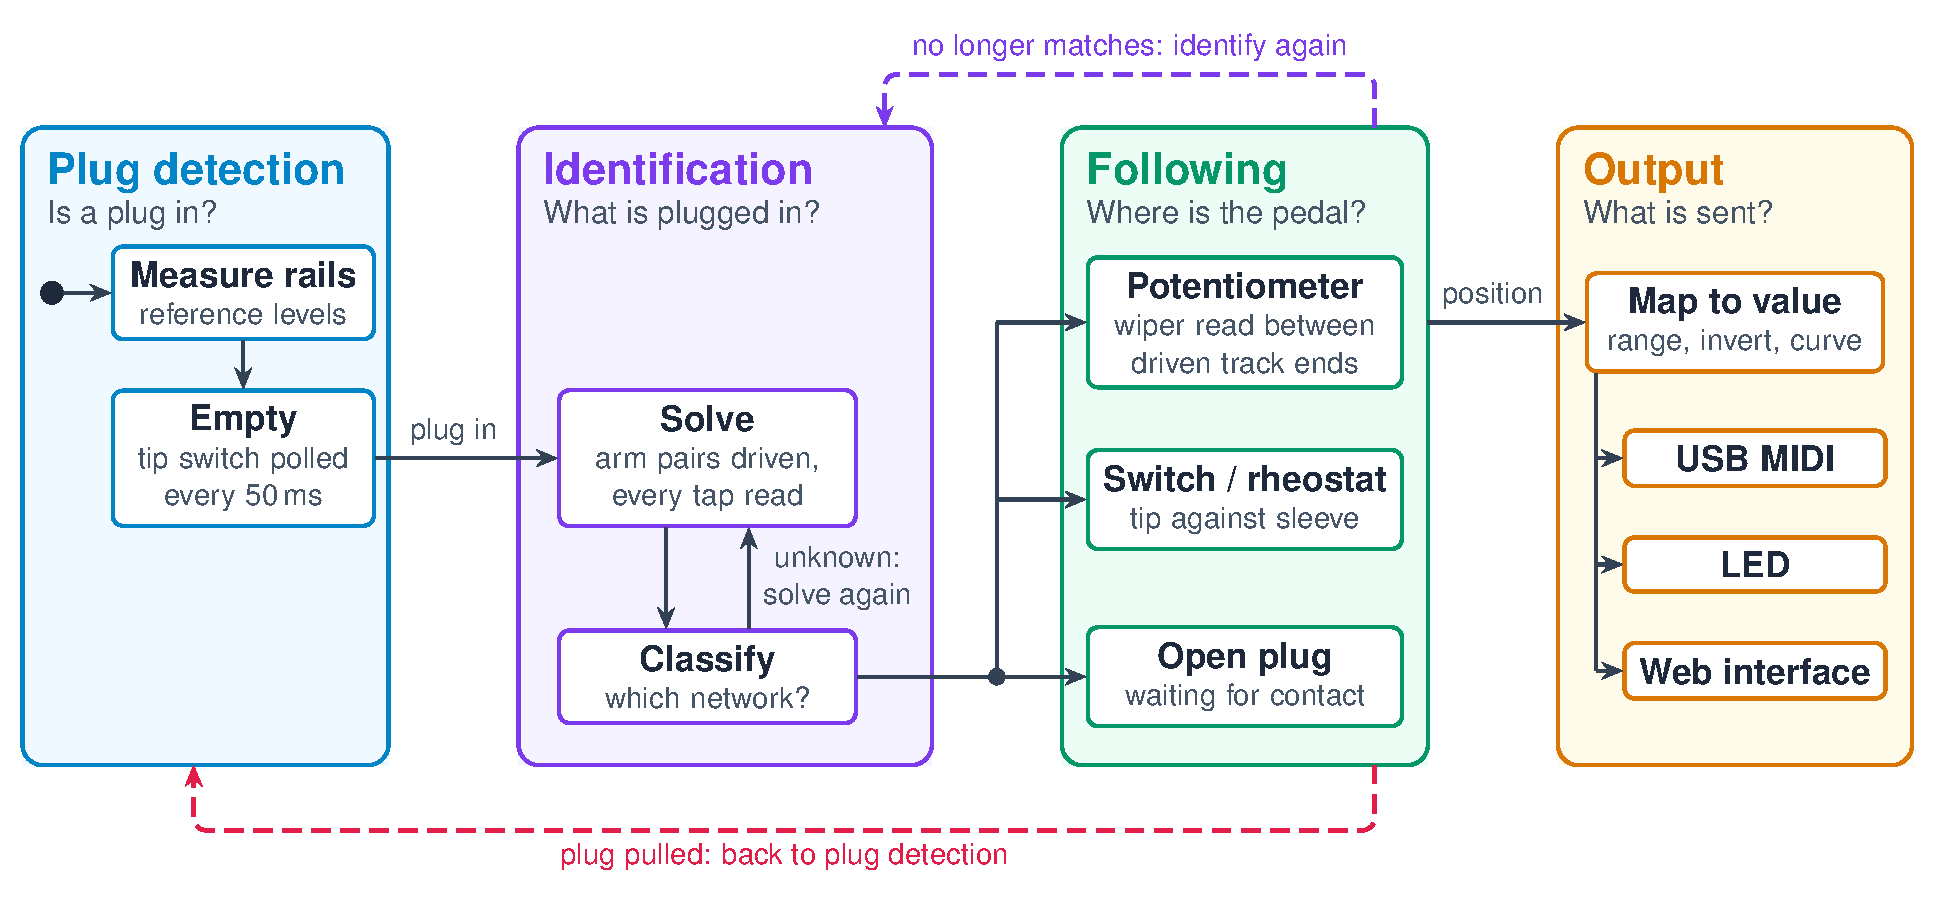
\includegraphics[width=\linewidth]{04-implementation/figures/jack-monitor-overview}
  \titledcaption{Firmware Overview}{\scaffoldinline{Name the four stages per jack (plug detection, identification, following, output) and the two ways back (re-identification when the pedal no longer matches, plug detection when the plug is pulled). Source: \code{docs/diagrams/jack-monitor-overview.tex}.}}
  \label{fig:firmware-overview}
\end{figure}

\scaffold{
  \textbf{Paragraph 3, development on the host.} The solver was first developed in an interactive simulator in TypeScript, shown at milestone~2 \cite{benson2026topologysim}, and then ported to Rust. Because \code{expad-topology} has no hardware dependency, it compiles for the host, where its tests drive the solver against a simulated star network and the state machine against a simulated jack in simulated time (52 tests at the final state, covering plugging, unplugging, end stops, mono and stereo plugs, switches, rheostats, resistive wipers and noise). Give the example that justified this effort: the tests ported from the simulator showed that the first port drove the pairs with high and low swapped, which half of the tests detected before the code ever ran on hardware. Every later solver fix in this report came with a test that fails without it.
}

\scaffold{
  \textbf{Paragraph 4, board-level tools.} Besides the controller firmware, the repository contains small programs that each run on the board alone, the most important being the pin-mapping self-test (\cref{sec:results-self-test}), a capture tool that holds a drive pattern and records every ADC input, and the ADC characterization of \cref{sec:update-rate}. Refer to \cref{tab:binaries} in the appendix for the full list.
}

% !TEX root = ../main.tex

\section{Jack Monitor}
\label{sec:jack-monitor}

\scaffold{
  \textbf{Paragraph 1, interface of the monitor.} One \emph{jack monitor} per jack implements \cref{sec:plug-detection,sec:following} as a state machine. It never touches hardware: it hands out one reading at a time (the drive of each of the four contacts, the contact to read, and whether the drive change needs settling) and takes the measured voltage back, together with the time in milliseconds. This lets a scheduler interleave jacks on two ADCs and lets the host tests drive it from a model. It reports a \emph{mode} per jack: empty, identifying, tracking (a potentiometer), switch, rheostat, open (a plug with nothing conducting), or other.
}

\scaffold{
  \textbf{Paragraph 2, states.} Walk through \cref{fig:jack-monitor-states} along the main flow: rails at start-up, empty with a plug check every \qty{50}{\milli\second}, solve (rails re-measured first if older than \qty{30}{\second}), classification, then one of the following states. Then the two ways back: following a potentiometer returns to identification when a track-end check or the wiper range fails, switch, rheostat and open return to empty when the plug check fails. Name the confirm-plug state, which tells an empty jack from an open plug after a solve found no current. Do not describe every edge; the figure does.
}

\begin{figure}[htbp]
  \centering
  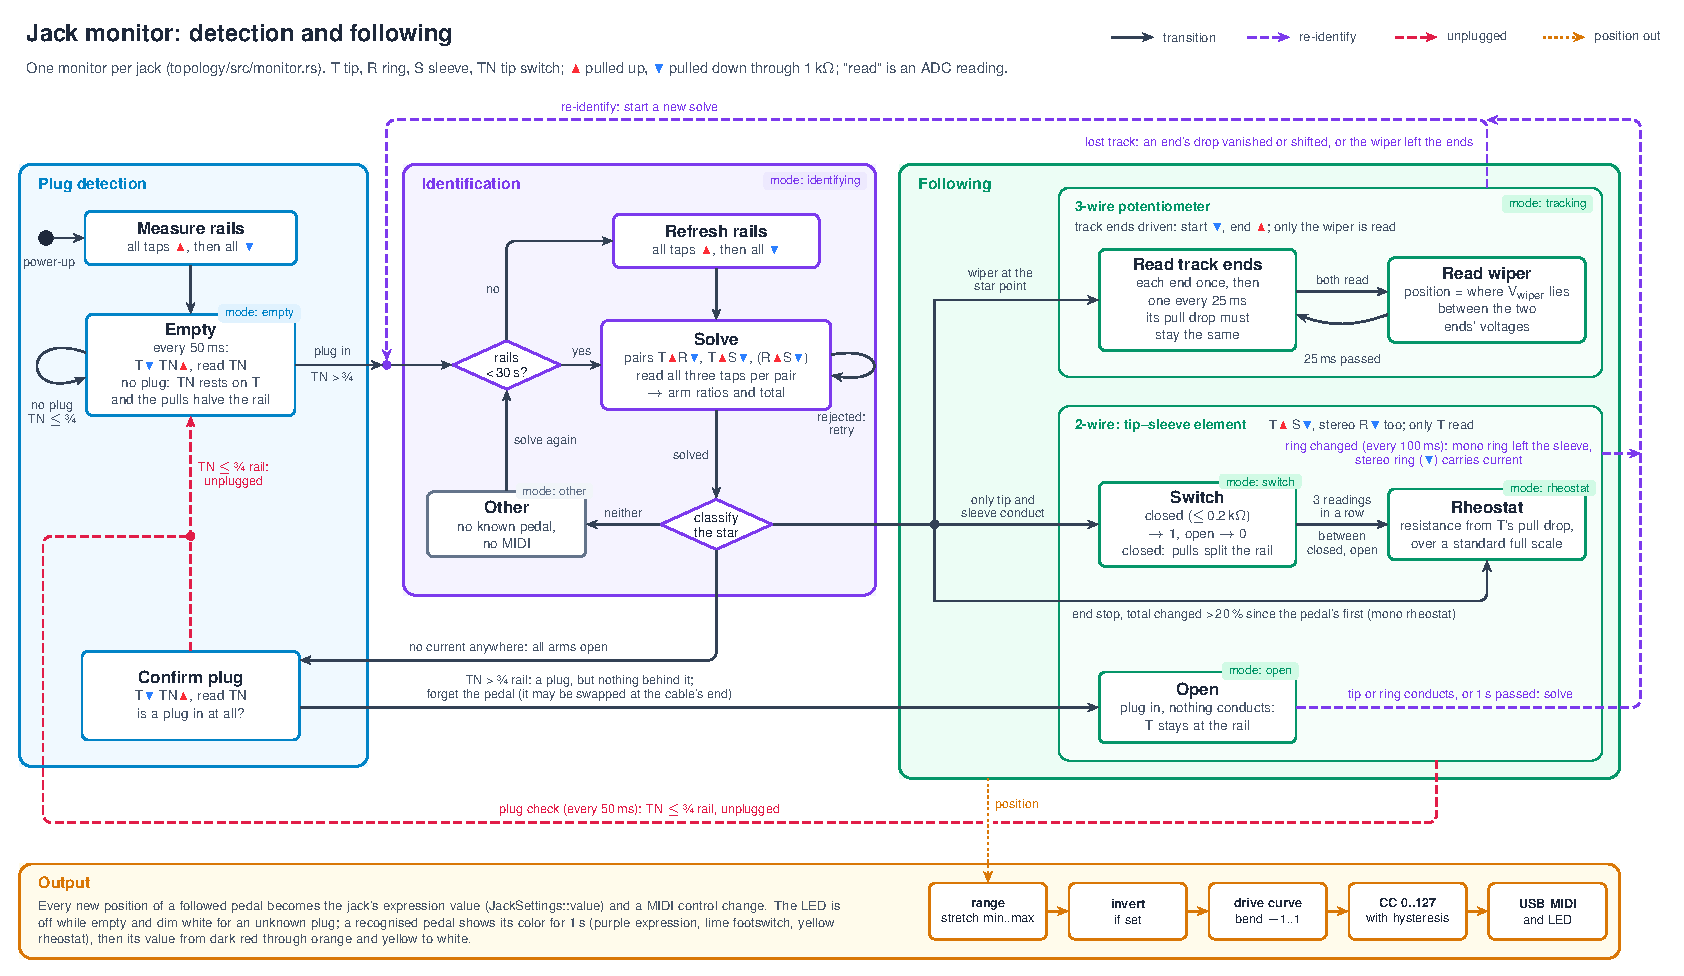
\includegraphics[width=\linewidth]{04-implementation/figures/jack-monitor-states}
  \titledcaption{Jack Monitor State Machine}{\scaffoldinline{Explain the three groups (plug detection, identification, following), the mode tag on each state, the drive symbols (red up, blue down), the two return corridors (re-identify above, unplugged below) and the output strip. Source: \code{docs/diagrams/jack-monitor-states.tex}. Consider a landscape page if the labels are too small at text width.}}
  \label{fig:jack-monitor-states}
\end{figure}

\scaffold{
  \textbf{Paragraph 3, constants.} Present \cref{tab:monitor-config} and point out that every interval and fraction was set or changed by an observation on the board; give two examples from the table with their reason (the \qty{25}{\percent} wiper limit from a pedal with resistance in its wiper lead, \cref{sec:pedal-types}; the \qty{25}{\percent} tolerance of the first track-end reading because solves of a pedal on an end stop were \qty{10}{\percent} off). The remaining reasons are in the appendix (\cref{tab:monitor-config-full}).
}

\begin{table}[htbp]
  \centering
  \titledcaption{Main Constants of the Jack Monitor}{\scaffoldinline{Explain that relative values refer to the total resistance of the network and that $\sigma$ is the noise of the checked quantity. Source: \code{MonitorConfig::new} in \code{topology/src/monitor.rs}.}}
  \label{tab:monitor-config}
  \begin{tabular}{@{}ll@{}}
    \toprule
    \textbf{Constant} & \textbf{Value} \\
    \midrule
    Plug check interval & \qty{50}{\milli\second} \\
    Track-end check interval (potentiometer) & \qty{25}{\milli\second} \\
    Ring check interval (switch, rheostat) & \qty{100}{\milli\second} \\
    Full solve of an open plug & every \qty{1}{\second} \\
    Rail refresh before a solve & after \qty{30}{\second} \\
    Readings averaged per rail & 8 \\
    Plug threshold & \num{0.75} of the rail span \\
    Largest wiper arm & \qty{25}{\percent} \\
    Largest arm at an end stop & \qty{2}{\percent} \\
    End-drop tolerance, first reading / later & \qty{25}{\percent} / \qty{3}{\percent} or $6\sigma$ \\
    Wiper range margin & $6\sigma$ + \qty{0.5}{\percent} of the span \\
    Closed switch & $\leq \qty{0.2}{\kilo\ohm}$ \\
    Readings between open and closed for a rheostat & 3 \\
    Assumed total before the first solve & \qty{100}{\kilo\ohm} \\
    \bottomrule
  \end{tabular}
\end{table}

\scaffold{
  \textbf{Paragraph 4, memory per plug.} What the monitor learns about a plug (that it is a rheostat, the total at its first end stop, the full scale) is forgotten when the plug comes out or turns out open, because a cable left in the jack may get the next pedal at its other end. The wiper of the last potentiometer is kept beyond that, for the next ambiguous end stop in the same jack. Mention the bug that motivated forgetting on an open plug: a stereo cable plugged into the jack first and into a potentiometer pedal afterwards connected tip and sleeve before the ring, was taken for a switch turning into a rheostat, and stayed one, until a ring check for stereo plugs was added.
}

% !TEX root = ../main.tex

\section{Scheduling and Update Rate}
\label{sec:update-rate}

\scaffold{
  \textbf{Paragraph 1, the starting point.} The first firmware on the PCB solved every jack in turn and needed \qty{382}{\milli\second} per sweep, so a pedal was updated 2.6 times per second; the user-facing target set during development was at least \qty{50}{\hertz}. Break the time down, which is the diagnosis: every reading changed the ADC channel and therefore paid three conversion periods (\cref{sec:conversion}), \qty{9.5}{\milli\second} at the initial \qty{315}{\hertz} plus about \qty{0.7}{\milli\second} of SPI traffic; every jack took nine readings (three pairs of three contacts), the empty ones included; four jacks $\times$ nine readings $\times$ \qty{10.3}{\milli\second} plus twelve settling waits of \qty{1}{\milli\second} gives the \qty{382}{\milli\second}. At \qty{50}{\hertz}, \qty{20}{\milli\second} buy about two readings, so no full solve can fit: speed had to come from reading faster and reading less.
}

\openquestion{Update-rate target}{
  Is the \qty{50}{\hertz} target a requirement of the project or a value chosen during development? The proposal only asks for \enquote{real time without perceptible latency}.
}

\scaffold{
  \textbf{Paragraph 2, reading faster: the ADC operating point.} A characterization program measured, on a \qty{10.85}{\kilo\ohm} potentiometer pedal held still in jack~1, the time per reading and the noise at five filter rates (\cref{tab:adc-characterization}). Draw the three conclusions: the output resolution scales with the cube of the filter word, as sinc\textsuperscript{3} decimation predicts ($(13/3)^3 \approx 81$ between the fastest and the slowest word), which rules out the fastest rate; continuous conversion on one channel is 2.5 to 3 times noisier at the fast rates and was not worth a separate code path; calibration does not carry over between filter words (the ground reading moved between \qty{-2.9}{\milli\volt} and \qty{+1.75}{\milli\volt}), so the firmware uses one rate for rails, solves and following. \qty{819}{\hertz} reads 2.3 times faster than \qty{315}{\hertz} at a noise of \qty{0.39}{\milli\volt}, which is the $\sigma_V = \qty{0.5}{\milli\volt}$ of \cref{sec:tolerances}. Mains hum of 100 to \qty{140}{\micro\volt} was present at every rate but amounts to about 60 parts per million of travel.
}

\begin{table}[htbp]
  \centering
  \small
  \titledcaption{ADC Characterization}{\scaffoldinline{State the conditions: \qty{10.85}{\kilo\ohm} pedal in jack~1, tip as wiper, ring high, sleeve low, bipolar coding, calibrated at every rate; \enquote{reading} includes the channel switch; position noise refers to the full travel. One MIDI step is \num{7874} parts per million. Source: \code{docs/fast-tracking.md}, program \code{adc\_characterization}.}}
  \label{tab:adc-characterization}
  \setlength{\tabcolsep}{4pt}
  \begin{tabular}{@{}rrrrrr@{}}
    \toprule
    \textbf{Rate} & \textbf{Filter word} & \textbf{Reading} & \textbf{Noise} & \textbf{Output step} & \textbf{Position noise} \\
    \textbf{(\unit{\hertz})} & & \textbf{(\unit{\milli\second})} & \textbf{(\unit{\milli\volt})} & \textbf{(\unit{\milli\volt})} & \textbf{(ppm)} \\
    \midrule
    1365 & 3 & 2.89 & 1.93 & 3.88 & 887 \\
    1024 & 4 & 3.63 & 0.80 & 0.41 & 374 \\
    819 & 5 & 4.36 & 0.39 & 0.21 & 203 \\
    682 & 6 & 5.09 & 0.40 & 0.12 & 184 \\
    315 & 13 & 10.22 & 0.11 & 0.012 & 62 \\
    \bottomrule
  \end{tabular}
\end{table}

\scaffold{
  \textbf{Paragraph 3, a solver weakness exposed.} At \qty{819}{\hertz} the sweep dropped to \qty{156}{\milli\second}, but the position noise rose instead of staying put. Cause: the test pedal has its wiper on the tip, which is the arm shared by the first two pairs, and with a contact resistance of \qty{1.5}{\percent} the conditioning (\cref{eq:conditioning}) was 0.083, just above the old minimum of 0.05; the solver then split the track through a few millivolts across the wiper and amplified the noise about 25-fold. Raising the minimum to 0.5 forces the third pair for such pedals. Present \cref{tab:conditioning-fix} and state that the flaw had already cost accuracy at \qty{315}{\hertz}; going faster only made it visible.
}

\begin{table}[htbp]
  \centering
  \titledcaption{Effect of the Minimum Conditioning}{\scaffoldinline{State the condition: pedal held still at position 0.21; sweep of all four jacks with full solves. Source: \code{docs/fast-tracking.md}.}}
  \label{tab:conditioning-fix}
  \begin{tabularx}{\linewidth}{@{}Xrrr@{}}
    \toprule
    \textbf{Configuration} & \textbf{Position (ppm)} & \textbf{Total} & \textbf{Sweep} \\
    \midrule
    \qty{315}{\hertz}, minimum 0.05 & 2588 & \qty{0.91}{\percent} & \qty{382}{\milli\second} \\
    \qty{819}{\hertz}, minimum 0.05 & 4880 & \qty{1.75}{\percent} & \qty{156}{\milli\second} \\
    \qty{819}{\hertz}, minimum 0.5 & 274 & \qty{0.11}{\percent} & \qty{171}{\milli\second} \\
    \bottomrule
  \end{tabularx}
\end{table}

\scaffold{
  \textbf{Paragraph 4, reading less.} The second and larger step was to stop re-solving an identified pedal: the jack monitor of \cref{sec:jack-monitor} follows it with one reading per update, which is the reason the state machine exists. Empty jacks cost one plug check every \qty{50}{\milli\second} instead of nine readings per sweep.
}

\scaffold{
  \textbf{Paragraph 5, scheduling on two ADCs.} The scanner gives each ADC to whichever of its two jacks is most overdue, applies the drives of both chosen jacks in one shift-register write, starts a conversion on both chips and waits for both. A followed jack keeps its drives while the other jack on the same ADC is read, so alternating between them costs no settling of the contacts, only the ADC's own three periods. Settling waits (\cref{eq:settling}) are only inserted when a drive actually changes. Finally, the SPI clock was raised from \qty{1}{\mega\hertz} to \qty{4}{\mega\hertz} and the chip-select guard cut from \qty{50}{\micro\second} to \qty{10}{\micro\second}, which shortened a reading from \qty{4.36}{\milli\second} to \qty{4.02}{\milli\second} without additional noise or outliers; three conversion periods alone take \qty{3.66}{\milli\second}. The resulting rates are evaluated in \cref{sec:results-update-rate}.
}

\scaffold{
  \textbf{Paragraph 6, two development bugs.} One sentence each, as examples of observations on the board that changed the design: a rejected solve made the firmware forget the pedal's resistance and fall back to the longest settling time, so a moving pedal was tracked in one direction only; and the first tracking check allowed only \qty{3}{\percent} deviation, which dropped pedals replugged on an end stop. Both are now covered by host tests.
}

% !TEX root = ../main.tex

\section{Output Stage}
\label{sec:output}

\scaffold{
  \textbf{Paragraph 1, from position to value.} The monitor reports a raw position $p$ (\cref{eq:position}); the per-jack settings turn it into the sent value in three steps, presented as \cref{eq:value-range,eq:drive-curve}: the range $[p_\mathrm{min}, p_\mathrm{max}]$, which the web interface sets from the current pedal position with two buttons, is stretched to $[0, 1]$ and clamped; the result is inverted if the jack is set to invert; then the drive curve bends it. Mention why the range exists: the test pedal only reached 0.909 of its track at the end of its travel, a mechanical stop common to pedals \cite{mission2014expression}.
}

\begin{align}
  u &= \operatorname{clamp}\!\left(\frac{p - p_\mathrm{min}}{p_\mathrm{max} - p_\mathrm{min}},\, 0,\, 1\right),
  \qquad u' = \begin{cases} 1 - u & \text{if inverted} \\ u & \text{otherwise} \end{cases}
  \label{eq:value-range} \\
  y &= \frac{(1 + b)\,u'}{1 - b + 2b\,u'},
  \qquad b = 0.9\,d, \qquad d \in [-1, 1]
  \label{eq:drive-curve}
\end{align}

\scaffold{
  \textbf{Paragraph 2, the drive curve.} \Cref{eq:drive-curve} is Schlick's bias function \cite{schlick1994bias} with the parameter $a = (1 + b)/2$; show this substitution in one line. Explain its three properties that made it the choice for a single knob $d$: both ends of the travel stay in place, half travel maps to $(1 + b)/2$, so the knob reads as where the pedal's midpoint lands, and $-d$ gives the exact inverse of $+d$, so one knob can straighten a pedal with a logarithmic potentiometer as well as one with an antilogarithmic one \cite{mission2014expression}. It needs no power function, which matters on a microcontroller without a math library. Example from the development: a logarithmic potentiometer that reads \qty{10}{\percent} at half travel is linearized at $d \approx 0.89$.
}

\begin{figure}[htbp]
  \centering
  \placeholderfigure[0.6\linewidth]{
    \textbf{Content.} $y$ over $u'$ from \cref{eq:drive-curve} for $d = -1, -0.5, 0, 0.5, 1$, square plot, equal axes from 0 to 1.
    \textbf{Focus.} Mark the point at $u' = 0.5$ on each curve with its value $(1 + 0.9d)/2$, and draw the curves for $\pm d$ in the same color with solid and dashed line to show that they are mirror images.
    \textbf{How to obtain.} Add a function to \code{measurements/create\_plots.py} (matplotlib, same style as the other plots); the formula is \code{drive\_curve} in \code{src/web/interface.rs}.
  }
  \titledcaption{Drive Curve}{\scaffoldinline{Name the parameter values and the meaning of the marked midpoints and of the mirror pairs.}}
  \label{fig:drive-curve}
\end{figure}

\scaffold{
  \textbf{Paragraph 3, MIDI.} The device enumerates as a class-compliant USB MIDI device \cite{usbif1999midi}, so no driver is needed. Each jack sends its value as a 7-bit control change, by default on MIDI channel 1 with controller 11 (expression) for jacks 1 and 2 and controller 1 (modulation wheel) for jacks 3 and 4 \cite{midi2026controlchange}. A new value is sent only when the rounded value changes and the value has moved by more than 0.6 of a step since the last sent one, which suppresses toggling between two neighbouring values. If the host is not reading, a newer value replaces the one still waiting, so no queue builds up and a host that connects receives every pedal's current position.
}

\scaffold{
  \textbf{Paragraph 4, USB robustness.} Two problems surfaced on a macOS host, and both are worth a sentence because they explain design choices of the driver. The device froze completely on connection: macOS reads the manufacturer string during enumeration, which was longer than the 64-byte control buffer of the USB stack allows, and the resulting panic halted the core (Windows never asked for it). Fix: a \qty{256}{\byte} control buffer and a check of the strings at start-up. In addition, embassy-rp~0.10 reported a suspend from before the bus reset, which can stall enumeration \cite{embassy2026pr6693}, and its writes do not end when the host disconnects \cite{embassy2024issue3426}; the firmware wraps the driver to clear the stale suspend, pace event floods, and end transfers on disconnection, and runs USB in its own tasks so that it can never stall the measurement.
}

\scaffold{
  \textbf{Paragraph 5, LEDs.} Each jack has an RGB LED below it, colored from the jack's mode and sent value: off when empty, dim white for a plug that is not (yet) a known pedal, a pedal-specific color for \qty{1}{\second} once per plug-in (purple for an expression pedal, lime for a switch, yellow for a rheostat), then the value as a gradient from dark red through red, orange and yellow to white. One sentence on the purpose: the user sees without a computer that a pedal was recognized and what it sends.
}

% !TEX root = ../main.tex

\section{Web Interface}
\label{sec:web-interface}

\scaffold{
  \textbf{Paragraph 1, access point and protocol.} The Pico~2~W opens a WPA2-protected WiFi access point and runs a DHCP server, a DNS server that answers every name with the device's address, and an HTTP server. Every path other than the interface itself is redirected to it, so phones and laptops open the interface as the sign-in page of the network (captive portal). The page holds a WebSocket connection: the device sends the status of every jack (mode, raw position, value, arm resistances, voltage and drive of every contact) about 30 times per second and the settings on every change; every settings message from a browser is applied and forwarded to all other open pages. Settings are not stored in flash yet, so they reset with every power cycle.
}

\scaffold{
  \textbf{Paragraph 2, the interface.} Describe \cref{fig:web-interface}: the jacks laid out as channel strips of a mixing desk, each with MIDI channel, controller, invert, range with minimum and maximum buttons, wiper setting and drive knob; and the side panel that draws the identified network of the selected jack with every pull switch, the measured contact voltages and a three-line explanation of what the jack is doing now, why, and what it waits for. State its role in the project in one sentence: it was the main debugging tool during development and made the classification visible during the demonstration.
}

\begin{figure}[htbp]
  \centering
  \placeholderfigure{
    \textbf{Content.} Screenshot of the web interface with four channel strips and the topology panel open on a jack that follows a potentiometer pedal.
    \textbf{Focus.} Crop to the strips and the panel; mark (numbered callouts) the range slider with its minimum and maximum buttons, the drive knob, the wiper setting, the drawn network with the identified wiper, and the explanation text.
    \textbf{How to obtain.} Either connect to the device (\code{npm run dev} in \code{web/}) with a pedal plugged in, or run \code{npm run dev:mock}, which simulates a potentiometer, a switch and a scripted plug-in sequence; take the screenshot in the browser at a window width of about 1600 pixels.
  }
  \titledcaption{Web Interface}{\scaffoldinline{Explain each numbered callout and which jack and pedal the screenshot shows.}}
  \label{fig:web-interface}
\end{figure}

\scaffold{
  \textbf{Paragraph 3, implementation in one sentence each.} The front end is a Vue single-page application built with Vite, Tailwind CSS and PrimeVue; the build step of the firmware compiles it into one gzipped HTML file that is embedded in the firmware image. A mock device that speaks the same protocol allows developing the interface without hardware. Do not go further into the web stack; it is not the subject of the report.
}

\openquestion{Android tablet drops}{
  WebSocket connections to one Android tablet dropped repeatedly (unacknowledged frames at the radio level) while other devices stayed connected; the captive portal was added in the hope of reducing the tablet's background scanning. Did it help? If the issue remains, mention it as a limitation in \cref{ch:discussion}.
}

